\documentclass[preprint,12pt]{elsarticle}

\usepackage[T1]{fontenc}
\usepackage{amsmath,amssymb,bm}
\usepackage{booktabs}
\usepackage{tabularx}
\usepackage{array}
\usepackage{pifont}
\usepackage{graphicx}
\usepackage{algorithm}
\usepackage{algpseudocode}
\usepackage[section]{placeins}
\usepackage{tikz}
\usetikzlibrary{arrows.meta,positioning,calc}
\usepackage[hidelinks,breaklinks]{hyperref}
\usepackage{xurl}

\newcolumntype{Y}{>{\raggedright\arraybackslash}X}
\newcolumntype{C}{>{\centering\arraybackslash}p{0.95cm}}
\newcommand{\code}[1]{\texttt{\detokenize{#1}}}
\newcommand{\N}{\mathcal{N}}
\newcommand{\E}{\mathbb{E}}
\newcommand{\R}{\mathbb{R}}
\newcommand{\zg}{\mathbf{z}_{g}}
\newcommand{\zl}{\mathbf{z}_{\ell}}
\newcommand{\bx}{\mathbf{x}}
\newcommand{\by}{\mathbf{y}}
\newcommand{\bz}{\mathbf{z}}
% Check/cross table marks
\newcommand{\yes}{\ding{51}}
\newcommand{\no}{\ding{55}}

\setlength{\emergencystretch}{2em}

\journal{Computer Methods in Applied Mechanics and Engineering}

\begin{document}

\begin{frontmatter}

\title{Generative mesh graph networks for imperfection-driven scatter in structural response fields}

\author{(authors)}

\begin{abstract}
When some inputs of a manufactured structure are not measured, such as its geometric
imperfections, one nominal design does not give one response. The same drawing gives a scatter
of response fields, and a surrogate model has to reproduce that scatter, not only its mean.
Field surrogates in computational mechanics are deterministic. Generative surrogates on meshes
exist, but most reproduce the time variation of turbulent flows, and none of the generative
surrogates of input scatter has been checked for sample realism, distribution match and
out-of-range inference together. We present HI-MGN-V, a hierarchical
mesh graph network that generates complete displacement fields on unstructured finite-element
(FE) meshes from the nominal design. A multilevel (V-cycle) graph network with 15 blocks is
adjusted before every block by a random latent vector. During training the latent vector is
inferred from the FE result; at prediction time it is drawn from a learned distribution
conditioned on the design. The latent vector can be one vector for the whole structure
(global), a field over coarse regions (local), or both (hybrid); the three options are three
assumptions about how the unmeasured input acts on the response. We compare the predicted
scatter with 1000 new FE analyses of the same nominal design on three criteria: (a) sample
realism, every generated field is close to some FE result and every FE result to some
generated field, measured by the nearest-neighbour $R^2$ in both directions; (b) distribution
match, the generated fields as a set are distributed as the FE results, measured by the
Wasserstein distance $W_2$ between the two sets of fields against the value that FE results
alone reach; and (c) out-of-range inference, (a) and (b) hold for designs outside the training
range. The test problem is an axially compressed cylindrical shell with 64 imperfection samples
per training geometry, in which the same nominal shell either stays unbuckled or buckles. Earlier
implementations of the global and local options fail in opposite ways: the local model has the
right mean but too little scatter, and the global model underestimates the displacement and
predicts too few buckled shells near the critical load. Results of the unified implementation
are pending and are not reported here.
\end{abstract}

\begin{keyword}
response scatter \sep geometric imperfection \sep generative surrogate model \sep mesh graph
network \sep shell buckling \sep flow matching
\end{keyword}

\end{frontmatter}

%======================================================================
\section{Introduction}\label{sec:intro}

\subsection{Motivation}

A finite-element model is deterministic once every input is given. In practice some inputs are
never given. The as-built geometry of a thin shell differs from the drawing by imperfections of
a fraction of the wall thickness. A fabricated part carries process variation, and a bolted
joint has an unknown preload. We write $\xi$ for such an input: a property of the individual
part that affects the response but is not part of the nominal design and is not available to
the analyst. A designer who works from the nominal design $c$ therefore faces one design with
many possible responses,
\begin{equation}
  \by = S(c,\xi),\qquad \xi\sim p(\xi),
\end{equation}
where $S$ is the FE solver and $\by$ the response field. The quantity of interest is the
conditional distribution $p(\by\mid c)$: the scatter of $\by$ obtained by running the solver
over the distribution of $\xi$ for a fixed design $c$.

Imperfection-sensitive structures make this scatter consequential. The axially compressed
cylindrical shell is the classical case: its buckling load is controlled by imperfections that
are small compared with the wall thickness, and the same shell can stay unbuckled or buckle
\cite{hutchinson1970postbuckling}. A designer reads statistics of scalar quantities of interest
(QoIs) from such a scatter, for example of the peak displacement magnitude $s=\max_i\|u_i\|$,
the probability that the shell buckles, or the location of the buckle. Repeated FE analyses
give these statistics at a cost of the number of designs times the number of imperfection
samples per design. A surrogate that generates complete response fields from $c$ and a random
input removes the inner loop.

Three properties make the target hard to learn. A surrogate trained with a squared-error loss
predicts the mean response, which for a shell near its critical load lies between the
unbuckled and the buckled state and is not itself a possible response. Generating possible
responses is not enough either: they must occur as often as in the FE results, and reproducing
the scatter of each node separately does not ensure that the whole field is distributed as in
the FE results, on which a QoI such as $s$ depends. And a design study goes beyond the
training data, so a surrogate has to be checked on designs it was not trained on, including
designs near the critical load, where $p(\by\mid c)$ changes fastest.

\subsection{Existing surrogates and the source of their scatter}

\paragraph{Deterministic field surrogates} Most surrogates of field solutions in computational
mechanics return one field per design. Projection-based and machine-learning-based reduced
order models have been built for nonlinear aeroelasticity \cite{lee2020time}, parametric flow
fields \cite{lee2021parametric}, fluid--structure interaction \cite{lee2024fsi,lee2024thesis},
nonlinear parametric problems with a deep hierarchical variational autoencoder used as a
compressor \cite{lee2024hvae}, and electromagnetic analysis of coated components
\cite{lee2025physics}. Mesh graph networks treat the simulation mesh as a graph and exchange
information between connected nodes \cite{gilmer2017neural,battaglia2018relational,pfaff2021mesh};
multiscale variants reach distant nodes through coarsened meshes
\cite{fortunato2022multiscale,cao2023efficient,lee2026himgn}, and combined local and global
attention has been used for the mechanical response of structures
\cite{patrignani2026hybrid}. Operator networks map input functions to output functions
\cite{lu2021learning,li2023fourier}. All of these return the mean response or a single field
per design. They have no mechanism for $\xi$.

\paragraph{Generative surrogates of turbulent and chaotic flows} Generative models of physical
fields exist, but nearly all of them reproduce the time variation of a turbulent or chaotic
system. Latent diffusion graph networks generate states of fully developed flows on meshes
\cite{lino2025distributions}; scale-autoregressive generation \cite{lino2026sar} and graph flow
matching \cite{song2026pifm} do the same; diffusion models generate turbulent states
\cite{lienen2024turbdiff,molinaro2024gencfd,liu2024uncertainty}; and ensemble weather models
generate future atmospheric states \cite{price2025gencast,oskarsson2024graphefm,alet2025fgn}.
In most of these problems the scatter comes from time: the reference data are the states of a
long simulation, and every condition has many states by construction. The exceptions hide a
small random perturbation of the initial condition or a random forcing
\cite{molinaro2024gencfd,park2026dll}, on regular grids and without a per-sample check of
realism or a test outside the training range. A shell with an unmeasured
imperfection is different. The solver is deterministic once $\xi$ is given, the response is one
static end state, and the scatter appears only because $\xi$ is not known.

\paragraph{Surrogates of input scatter} Stochastic emulators model the scatter of a response as
a function of the input, from repeated runs at the same input: generalized lambda models and
stochastic polynomial chaos for scalar QoIs \cite{zhu2021glam,zhu2023spce,zhu2023seismic} and
spectral surrogates for functional outputs \cite{luthen2023spectral}. In mechanics and design,
conditional generative models have been applied to structural strain fields under random loads
\cite{silionis2024deep}, to fabrication variation \cite{azimi2026genfab}, to geometric
uncertainty of metamaterials \cite{zheng2026gust}, and to multimodal and bifurcating responses
\cite{han2026multimodal,hendriks2025equivariant,zimmel2026bifork}. These works already address
parts of the problem studied here. Section~\ref{sec:position} compares them property by
property; none of them combines an unmeasured input, a high-dimensional field on an
unstructured mesh, and a comparison with many FE results per design on the three criteria
below.

\subsection{Research gap}

A generative surrogate of input scatter has to be compared with many FE results of the same
design. We use three criteria.
\begin{description}
\item[(a) Sample realism.] Each generated field should be close to some FE result of the same
  design, and each FE result should be close to some generated field. A model can match the
  mean and the standard deviation at every node with fields that no FE analysis would produce,
  for example fields between the unbuckled and the buckled state. The check is made sample by
  sample, so it does not weigh how often each kind of field occurs.
\item[(b) Distribution match.] The generated fields of a design, taken as a set, should be
  distributed as the FE results: how often the shell buckles, where and how strongly, and how
  all nodes vary together. A model that generates buckled fields for nine draws in ten where
  the FE analyses buckle in four can pass (a) in both directions and fails (b); a model that
  matches the scatter node by node can still fail (b), because a QoI such as the peak
  displacement depends on the whole field.
\item[(c) Out-of-range inference.] (a) and (b) must hold for designs outside the training
  range, including designs near the critical load, where the buckling probability changes
  fastest.
\end{description}
To our knowledge, no generative surrogate of structural response fields has been evaluated on
all three (Table~\ref{tab:ox}). Among the generative surrogates whose scatter comes from an
unobserved input, none checks (a) and (b) together, and none checks (c).

\subsection{Contributions}

\begin{enumerate}
\item \textbf{Problem definition and comparison with prior work.} We separate scatter caused by
  an unmeasured input from the time variation of turbulent flows and compare the closest prior
  work on the source of the scatter, the unmeasured input, the availability of several results
  per model input, and criteria (a)--(c) (Section~\ref{sec:related}, Table~\ref{tab:ox}).
\item \textbf{HI-MGN-V.} A hierarchical mesh graph network that generates complete response
  fields on unstructured meshes. A random latent vector adjusts every block of a V-cycle graph
  network and is drawn from a conditional distribution that is fitted after the rest of the
  model is frozen. Where the latent vector acts (global, local or hybrid) is an assumption about
  how $\xi$ acts on the field, and it is one switch in one implementation
  (Section~\ref{sec:method}).
\item \textbf{An evaluation protocol.} 1000 new FE results per evaluation design as the
  reference; a posterior-versus-prior check that locates failures; statistics of scalar QoIs;
  sample realism as the nearest-neighbour $R^2$ between generated and FE fields in both
  directions; distribution match as the Wasserstein distance $W_2$ between the generated and
  the FE fields; each score beside the value reached by FE results alone; on unseen,
  near-critical and out-of-range designs (Section~\ref{sec:metrics}).
\item \textbf{A shell-buckling dataset} with 64 imperfection samples for each of 150 geometries
  and 8 out-of-range geometries, in which the imperfection decides whether the shell buckles
  (Section~\ref{sec:dataset}).
\end{enumerate}

\paragraph{Scope} The scatter studied here comes from an unmeasured input, not from time
variation. The solver is deterministic once $\xi$ is given, and the response is one static end
state, not a time history. One dataset is used. The results of earlier implementations in
Section~\ref{sec:prelim} motivate the method; results of the unified implementation are
pending.

%======================================================================
\section{Related work}\label{sec:related}

\subsection{Deterministic field surrogates}

MeshGraphNets \cite{pfaff2021mesh} encode a mesh as nodes and edges, process it with residual
message-passing blocks, and map the node features to the outputs. Multiscale versions coarsen the mesh to pass
information further per block \cite{fortunato2022multiscale}; bi-stride pooling builds the
coarse levels from the connectivity \cite{cao2023efficient}; and HI-MGN combines configurable
coarsening with learned interpolation from neighbouring coarse nodes \cite{lee2026himgn}.
Patrignani and Pinho add combined local and global attention to graph networks for structural
response \cite{patrignani2026hybrid}. Their global path passes information across the
structure deterministically. A global random vector and a global information path are
different mechanisms, and Section~\ref{sec:placement} keeps them apart. Reduced order models
compress parametric solutions into a few coefficients
\cite{lee2020time,lee2021parametric,lee2024fsi,lee2024hvae,lee2025physics,lee2024thesis};
the variational autoencoder in \cite{lee2024hvae} serves as a compressor and the surrogate is
used deterministically. The graph network inside HI-MGN-V is the HI-MGN V-cycle.

\subsection{Stochastic emulators of input scatter}

Stochastic emulation treats the response at a given input as a random variable and learns its
distribution from repeated runs. Generalized lambda models and stochastic polynomial chaos
model the distribution of a scalar QoI \cite{zhu2021glam,zhu2023spce}, including seismic
structural response \cite{zhu2023seismic}. Spectral surrogates built from repeated time
histories extend this to functional outputs \cite{luthen2023spectral}. These works establish
the evaluation logic used here: repeated runs at the same input are the reference. They are not
designed for fields on varying meshes with tens of thousands of nodes.

\subsection{Generative surrogates of turbulent and chaotic flows}

Latent diffusion graph networks (LDGN) generate states of fully developed flows from a
compressed latent field on a coarse mesh \cite{lino2025distributions}. They are trained on
short simulations and compared, with a Wasserstein distance over the whole field, with the
states of long simulations; their appendix also trains latent flow matching.
Scale-autoregressive generation (SAR) generates the field coarse level first and refines it
level by level \cite{lino2026sar}, and PIFM-GN trains graph flow matching in physical and
latent space \cite{song2026pifm}. Diffusion models generate turbulent states
\cite{lienen2024turbdiff,molinaro2024gencfd} and flow uncertainty around airfoils
\cite{liu2024uncertainty}; GenCast, Graph-EFM and FGN generate ensemble weather forecasts
\cite{price2025gencast,oskarsson2024graphefm,alet2025fgn}. These methods are the technical
precedents for generating fields on meshes, and in most of them the scatter is the time
variation of a turbulent state, not an unmeasured static input. Two exceptions hide an input.
GenCFD trains on flows whose initial conditions carry small random perturbations and compares
its samples with many solver runs per macroscopic condition \cite{molinaro2024gencfd}, and
distributional operator learning with a diffusion last layer is trained on stochastic Burgers
and Darcy problems with random forcing or source terms, several solutions per input, and is
scored with an energy distance over the whole field \cite{park2026dll}; proper scoring rules
serve the same purpose for neural operators \cite{bulte2025pno}. Both work on regular grids, and
neither scores the realism of each sample nor tests the scatter outside the training range.

\subsection{Generative models of input scatter in mechanics and design}

Several works are close to this paper and rule out a claim that the problem is untreated.
Silionis et al.\ train a CVAE \cite{kingma2014vae,sohn2015cvae} for strain fields of a plate
and a ship hull under random loads \cite{silionis2024deep}. The loads are not model inputs, so
the model has to reproduce their effect as scatter; each FE run has its own thickness and load,
and the reference statistics are pooled over the test set. Yang and Perdikaris train
conditional implicit generators for stochastic systems \cite{yang2019conditional}, and
engression trains a generator with a proper scoring rule
\cite{shen2025engression,pacchiardi2024scoring}. Gen-Fab predicts fabrication variation of
nanophotonic devices and tests designs outside its training set \cite{azimi2026genfab}. GUST
quantifies free-form geometric uncertainty of metamaterials from small data and passes
generated shapes through a solver \cite{zheng2026gust}. Han and Bahmani learn pointwise
conditional mixture densities of multimodal responses, for a bifurcation normal form with a
bounded imperfection and a one-dimensional reaction--diffusion equation with random initial
conditions \cite{han2026multimodal}. Equivariant flow matching generates alternative
symmetry-breaking solutions, including buckled configurations of a beam
\cite{hendriks2025equivariant}, and Bi-FORK generates solution paths on distinct bifurcation
branches of a metamaterial and of an Allen--Cahn problem with random initial noise
\cite{zimmel2026bifork}. Each of these covers some of the properties in Table~\ref{tab:ox}. The
present paper is the combination: an unmeasured input, a static field on an unstructured mesh,
structural mechanics, and many FE results per design, compared on (a)--(c).

\subsection{Positioning}\label{sec:position}

Table~\ref{tab:ox} marks each property as met (\yes) or not (\no); a property that is met in
part, or not reported, is \no. \emph{Cause of scatter} names what produces the spread of the
reference data: a random initial condition, load, forcing or imperfection, a bifurcation into
several solutions, or the evolution of a turbulent state in time (temporal). Deterministic
surrogates return one field per design and are left out. \emph{Unobserved input} is met when the
scatter is caused by an explicitly stated physical or numerical random input whose realization
the model does not receive. The phase of a time series and a branch label are not such inputs.
\emph{Several results per input} is met when the data contain several solver results
for the same model input, so that the predicted scatter can be compared with the solver scatter
input by input instead of pooled over inputs. The states of one long simulation count; mirrored
copies of one solution and results at different loads do not. Columns (a)--(c) are the three
criteria of the research gap, graded strictly: (a) sample realism is met only when every
generated sample is scored quantitatively against the reference, by an error to the nearest
reference result, a residual or a validity rate, not by figures or by the mean and standard
deviation of the ensemble; (b) distribution match is met only when the distribution of whole
fields is compared, by a distance between field distributions (Wasserstein, energy distance,
MMD), a covariance or a variogram, not by per-node statistics, mode frequencies or spectra
alone; and (c) out-of-range inference is met only when checks of the kinds required by (a) and
(b) are both repeated on inputs outside the training range.

\begin{table}[!htbp]
\centering
\scriptsize
\setlength{\tabcolsep}{2pt}
\begin{tabularx}{\textwidth}{@{}Y >{\raggedright\arraybackslash}p{2.5cm} >{\raggedright\arraybackslash}p{2.1cm} *{5}{>{\centering\arraybackslash}p{1.1cm}}@{}}
\toprule
Work & Method & Cause & Unobs. & Several & (a) & (b) & (c) \\
 & & of scatter & input & results & Sample & Distrib. & Out-of- \\
 & & & & per input & realism & match & range inf. \\
\midrule
Yang \& Perdikaris, Burgers \cite{yang2019conditional} & VAE + GAN & initial condition & \yes & \yes & \no & \no & \no \\
CVAE, plate and hull \cite{silionis2024deep} & CVAE, CNN & load & \yes & \no & \no & \no & \no \\
Han \& Bahmani \cite{han2026multimodal} & MDN & imperfection, initial condition & \yes & \yes & \no & \no & \no \\
Gen-Fab, photonic device \cite{azimi2026genfab} & cGAN, U-Net & imperfection & \yes & \yes & \yes & \no & \no \\
GUST, printed unit cell \cite{zheng2026gust} & diffusion, U-Net & imperfection & \yes & \yes & \no & \no & \no \\
Equivariant FM, beam \cite{hendriks2025equivariant} & FM & bifurcation & \no & \no & \no & \yes & \no \\
Bi-FORK, metamaterial \cite{zimmel2026bifork} & AE + FM & bifurcation & \no & \no & \yes & \no & \no \\
Bi-FORK, Allen--Cahn \cite{zimmel2026bifork} & AE + FM & initial condition & \yes & \yes & \yes & \no & \no \\
\midrule
LDGN, EllipseFlow \cite{lino2025distributions} & VAE + diffusion, GNN & temporal & \no & \yes & \yes & \yes & \yes \\
SAR, EllipseFlow \cite{lino2026sar} & VAE + FM, GNN & temporal & \no & \yes & \yes & \yes & \yes \\
PIFM-GN, EllipseFlow \cite{song2026pifm} & FM, GNN & temporal & \no & \yes & \yes & \no & \no \\
Turbulence diffusion \cite{lienen2024turbdiff} & diffusion, U-Net & temporal & \no & \yes & \no & \no & \no \\
GenCFD, shear flow \cite{molinaro2024gencfd} & diffusion, U-Net & initial condition & \yes & \yes & \no & \no & \no \\
Airfoil diffusion \cite{liu2024uncertainty} & diffusion, U-Net & temporal & \no & \yes & \no & \no & \no \\
Diffusion last layer \cite{park2026dll} & neural operator + diffusion & forcing & \yes & \yes & \no & \yes & \no \\
\midrule
This work & VAE + FM, GNN & imperfection & \yes & \yes & \no & \no & \no \\
\bottomrule
\end{tabularx}
% Graded 2026-10-20 from the full texts (Silionis et al. from arXiv v1, 2302.08329). Dropped rows
% remain cited in Section 2: GLaM/SPCE, spectral surrogate, engression (scalar or design-space
% outputs), weather ensembles (scored against observations, not solver ensembles), PNO (read in
% full: all X; energy score against one observation). The first four were NOT re-read in full.
% Gen-Fab (2603.11505v1) and GUST (2506.12051v2) added back after a full read: Gen-Fab (a) rests
% on random-matching IoU (Sec. 3.2, Table 1); its W-D/KL-D are pixel-intensity histograms (b X);
% GUST W-D is per stiffness component (Sec. 4.5), density/coverage synthetic-only (b X).
\caption{Positioning. \yes: met and reported; \no: not met, met in part, or not reported. The
criteria are defined in Section~\ref{sec:position}. Method: the generative model, then the network
where the paper fixes one (AE autoencoder, FM flow matching, MDN mixture density network). Gen-Fab and GUST generate the as-fabricated
shape, not a response field, and name the fabrication process as the unobserved input without a
random parameter; Gen-Fab has replicates for its test designs only, scores each sample by its
overlap (IoU) with a fabricated replicate, and compares sets through pixel-intensity histograms;
GUST compares its response scatter through scalar homogenized stiffnesses only.
Several results per input from the
states of one simulation (LDGN, SAR, PIFM-GN, turbulence diffusion) are not independent
repetitions of an analysis. The equivariant-FM reference is one solution and its mirror image.
The airfoil-diffusion scatter is the pseudo-time of an unconverged solver, not a random input.
For this work, (a)--(c) are \no{} because no result of the unified model is reported yet; the
earlier implementations report only statistics of the scalar response $s$
(Section~\ref{sec:prelim}).}
\label{tab:ox}
\end{table}

\subsection{Where the random variable enters the model}

Generative models differ in where they put the latent variable. A \emph{global} latent is one
vector per sample: CVAEs, diffusion autoencoders \cite{preechakul2022diffae}, latent
task-specific graph simulators \cite{dahlinger2023ltsgns} and a variational graph autoencoder
for structural modal identification \cite{nath2026uresvgae}. A \emph{local} latent is attached
to positions or regions: the coarse-mesh latent of LDGN, spatially varying modulation in image
synthesis \cite{park2019spade,zhu2020sean,tan2021inade}, and the per-scale latents of
hierarchical segmentation models \cite{baumgartner2019phiseg,kohl2019hpunet}. \emph{Hybrid}
latents combine both: LION \cite{zeng2022lion}, PointFlow \cite{yang2019pointflow} and DualDiff
\cite{xie2026dualdiff}. The only controlled comparison of global, local and hierarchical
latents we found is in image segmentation (HPU-Net, its Appendix~F) \cite{kohl2019hpunet}.
Neither option is ruled out by theory: a global vector can carry a location through an
input-dependent expansion \cite{park2026dll}, and local multiscale computation can reproduce
long-range correlation \cite{masuki2026rgfm}. Two further findings shape the design. A
deterministic shortcut can bypass the random path \cite{baumgartner2019phiseg}, and feeding the
same random vector to every layer can help or fail depending on the design
\cite{park2019spade,karras2019stylegan,tan2021inade}.

\subsection{Latent regularization and evaluation scores}

The $\beta$-VAE trades reconstruction accuracy for agreement with the prior through a KL weight
\cite{higgins2017beta}. InfoVAE and the Wasserstein autoencoder replace the per-sample KL with a
distance between the distribution of all latent vectors and the prior, often an MMD
\cite{zhao2019infovae,tolstikhin2018wae,gretton2012kernel}. Regularized autoencoders and the
two-stage VAE fit a distribution to the learned latent vectors after training
\cite{ghosh2020rae,dai2019diagnosing}, as do diffusion autoencoders \cite{preechakul2022diffae};
LSGM shows that training the prior jointly can matter \cite{vahdat2021lsgm}. Proper scoring
rules are the basis for comparing a predicted distribution with observations
\cite{gneiting2007strictly}. The energy score is weak at detecting errors in correlation, and
variogram scores complement it \cite{scheuerer2015variogram,pic2024proper}. Rank histograms
show whether the scatter is too wide or too narrow \cite{hamill2001rank}, and precision,
recall, density and coverage separate whether individual samples are realistic from whether
the samples cover the reference scatter \cite{kynkaanniemi2019improved,naeem2020reliable}.
LDGN and SAR score each generated flow state by the $R^2$ to the nearest state of a long
reference simulation and compare the two sets of fields with a Wasserstein distance over the
whole field \cite{lino2025distributions,lino2026sar}; the present protocol follows them and adds
the reverse direction of the nearest-neighbour check. With a finite number of FE runs per
design, even a perfect model does not score zero \cite{luthen2023spectral,kansal2023evaluating}.

%======================================================================
\section{Method: HI-MGN-V}\label{sec:method}

\subsection{Problem statement}\label{sec:problem}

A sample is the FE mesh, treated as a graph $G=(V,E)$ with $N=|V|$ nodes and the element
edges as graph edges. The nominal input $c$ consists of the reference coordinates, the shell thickness $t$, the applied end shortening $\Delta$
(constant over nodes, stored per node) and a node type (interior, clamped rim, loaded rim). The
solver returns the displacement field $\by\in\R^{N\times3}$ at the end of loading. The unmeasured
input $\xi$ enters the solver's initial geometry but not $c$. In the dataset of
Section~\ref{sec:dataset}, $\xi$ is one Gaussian dimple with three random variables: its
amplitude, its angular position and its axial position. The training data are $M$ geometries
with $K$ imperfection samples each, $\{(c_m,\by_{m,k})\}_{k=1}^{K}$, and the imperfections
$\xi_{m,k}$ are not given to the model. The goal is a generator
\begin{equation}
  \hat\by = D(c,\bz),\qquad \bz\sim p_\theta(\bz\mid c),
\end{equation}
whose output scatter matches $p(\by\mid c)$ on geometries not used in training and on
geometries outside the training range. The latent vector $\bz$ is not an estimate of $\xi$: it
only has to describe the part of the effect of $\xi$ that is visible in the response field.

\subsection{Overview}

Figure~\ref{fig:arch} shows the model. It has three parts. A multilevel (V-cycle) graph
network $D$ maps the nominal input and a latent vector to a displacement field. During
training, an encoder $q_\phi(\bz\mid c,\by)$ infers the latent vector from the FE result. At
prediction time the FE result is not available, and the latent vector is drawn from a learned
distribution $p_\theta(\bz\mid c)$ that depends only on the nominal input. In the usual VAE
terminology, $q_\phi$ is the posterior and $p_\theta$ the prior. The placement setting
(global, local or hybrid) changes the size of $\bz$, which part of the encoder and of the
learned distribution produces it, and which part of $\bz$ each node reads. Nothing else
changes.

\begin{figure}[!htbp]
\centering
\resizebox{\linewidth}{!}{%
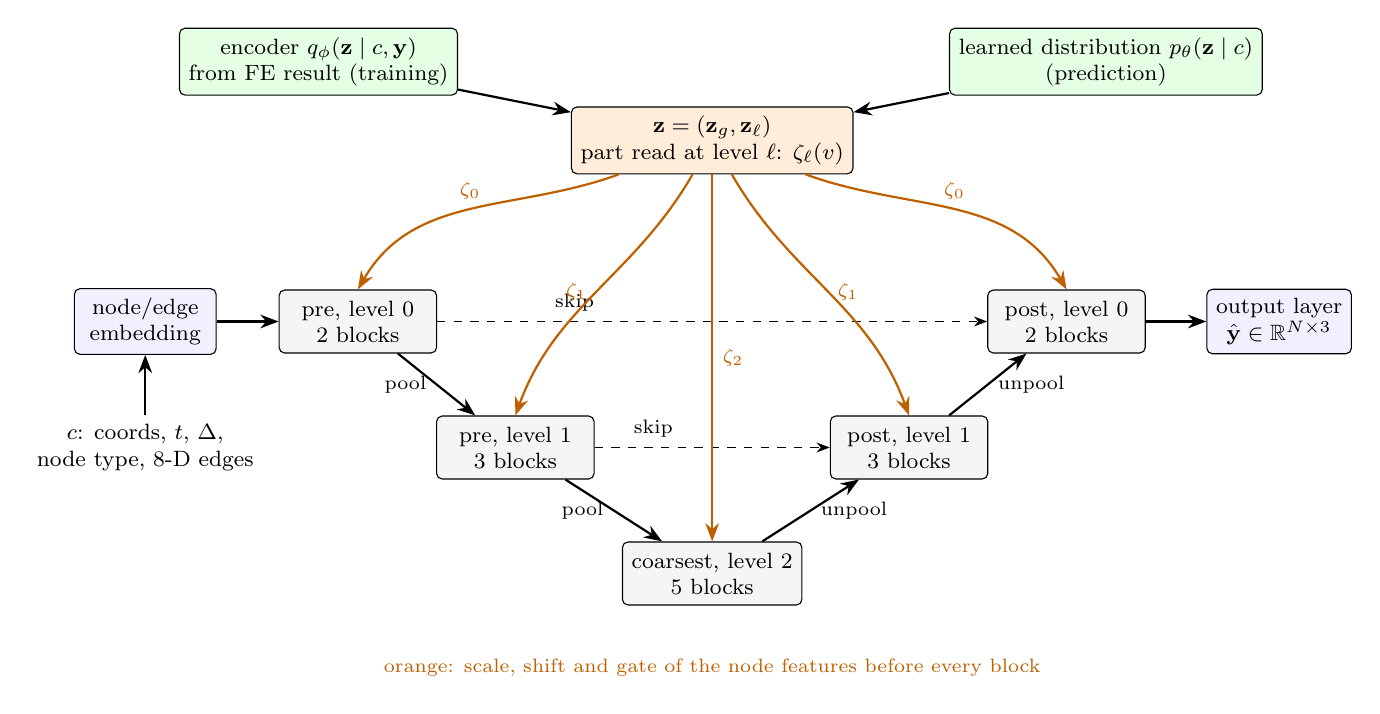
\begin{tikzpicture}[
  font=\footnotesize, >=Stealth,
  blk/.style={draw, rounded corners=2pt, align=center, minimum height=0.8cm, minimum width=2.0cm, fill=gray!8},
  io/.style={draw, rounded corners=2pt, align=center, minimum height=0.8cm, minimum width=1.8cm, fill=blue!6},
  zb/.style={draw, rounded corners=2pt, align=center, minimum height=0.8cm, fill=orange!15},
  mod/.style={->, thick, orange!75!black},
  fl/.style={->, thick}]
\node[io]  (enc) at (0,0)      {node/edge\\embedding};
\node[blk] (p0)  at (2.7,0)    {pre, level 0\\2 blocks};
\node[blk] (p1)  at (4.7,-1.6) {pre, level 1\\3 blocks};
\node[blk] (c2)  at (7.2,-3.2) {coarsest, level 2\\5 blocks};
\node[blk] (q1)  at (9.7,-1.6) {post, level 1\\3 blocks};
\node[blk] (q0)  at (11.7,0)   {post, level 0\\2 blocks};
\node[io]  (dec) at (14.4,0)   {output layer\\$\hat{\by}\in\R^{N\times3}$};
\node[align=center] (x) at (0,-1.6) {$c$: coords, $t$, $\Delta$,\\node type, 8-D edges};
\draw[fl] (x) -- (enc);
\draw[fl] (enc) -- (p0);
\draw[fl] (p0) -- node[left, font=\scriptsize] {pool} (p1);
\draw[fl] (p1) -- node[left, font=\scriptsize] {pool} (c2);
\draw[fl] (c2) -- node[right, font=\scriptsize] {unpool} (q1);
\draw[fl] (q1) -- node[right, font=\scriptsize] {unpool} (q0);
\draw[fl] (q0) -- (dec);
\draw[->, dashed] (p0.east) -- node[above, font=\scriptsize, pos=0.25] {skip} (q0.west);
\draw[->, dashed] (p1.east) -- node[above, font=\scriptsize, pos=0.25] {skip} (q1.west);
\node[zb] (z) at (7.2,2.3) {$\bz=(\zg,\zl)$\\part read at level $\ell$: $\zeta_\ell(v)$};
\node[zb, fill=green!10] (post) at (2.2,3.3) {encoder $q_\phi(\bz\mid c,\by)$\\from FE result (training)};
\node[zb, fill=green!10] (prior) at (12.2,3.3) {learned distribution $p_\theta(\bz\mid c)$\\(prediction)};
\draw[->, thick] (post) -- (z);
\draw[->, thick] (prior) -- (z);
\draw[mod] (z) to[out=200, in=60] node[above, font=\scriptsize] {$\zeta_0$} (p0.north);
\draw[mod] (z) to[out=240, in=70] node[left, font=\scriptsize] {$\zeta_1$} (p1.north);
\draw[mod] (z.south) -- node[right, font=\scriptsize] {$\zeta_2$} (c2.north);
\draw[mod] (z) to[out=300, in=110] node[right, font=\scriptsize] {$\zeta_1$} (q1.north);
\draw[mod] (z) to[out=340, in=120] node[above, font=\scriptsize] {$\zeta_0$} (q0.north);
\node[font=\scriptsize, orange!75!black, align=left] at (7.2,-4.4)
  {orange: scale, shift and gate of the node features before every block};
\end{tikzpicture}}
\caption{HI-MGN-V. The graph network is a 15-block V-cycle over three levels of one mesh
(fine mesh, 4096 clusters, 256 clusters). Before every block, the node features are scaled and
shifted by the part $\zeta_\ell(v)$ of the latent vector that the placement assigns to that
node at that level (Table~\ref{tab:placement}). During training the latent vector is inferred
from the FE result $\by$; at prediction time it is drawn from the learned distribution, which
sees only the nominal input. The graph network never sees $\by$.}
\label{fig:arch}
\end{figure}

\subsection{Graph inputs and hierarchy}\label{sec:graph}

Each node carries $[\,\text{state}\mid\text{conditions}\mid\text{position}\mid
\text{node type}\,]$: the state block (three displacement components, zero in this static,
single-step problem), the thickness and end shortening $(t,\Delta)$, four position features and
a three-way node-type indicator (interior, clamped rim, loaded rim). Each edge $(i,j)$ carries eight features, the relative position in
the current and in the reference configuration with their norms,
$[\,\mathbf{d}^{\text{cur}}_{ij},\|\mathbf{d}^{\text{cur}}_{ij}\|,
\mathbf{d}^{\text{ref}}_{ij},\|\mathbf{d}^{\text{ref}}_{ij}\|\,]$. In the static case the two
coincide. Every input and output component is scaled to zero mean and unit variance with
statistics of the training set.

The hierarchy has $L=2$ coarse levels with 4096 and 256 clusters. Seed nodes are spread
evenly over the mesh (farthest-point sampling), and every node is assigned to the nearest seed
along the mesh edges. A coarse node averages its members, and two coarse nodes are connected
when their clusters touch. Each fine node $v$ has an ancestor $a_\ell(v)$ at level
$\ell$ and a \emph{coarsest ancestor} $a_L(v)$. Two partitions with different random seeds are
prepared per training sample and one is drawn per visit; inference uses a fixed seed. The
partition is random, not a decomposition into physical regions.

\subsection{V-cycle graph network}\label{sec:vcycle}

Node and edge features are mapped to vectors of width $H=128$. The network has 15 blocks
distributed as $(2,3,5,3,2)$ over the fine level, level~1, level~2, level~1 and the fine level.
In each block every edge is updated from its two end nodes and every node from its edges, and
the result is added to the input of the block (message passing \cite{pfaff2021mesh}). Going
down, member features are averaged into the next coarser level. Going up, a fine node
interpolates from neighbouring coarse nodes with learned weights and adds the features it had at
the same level on the way down \cite{lee2026himgn}. A small fully connected network maps the
final fine-level features to the three displacement components. Without the latent vector, this
network is the deterministic HI-MGN.

\subsection{Latent placement: three assumptions about how $\xi$ acts}\label{sec:placement}

Where the latent vector acts states what the model assumes about the effect of $\xi$ on the
field.
\begin{itemize}
\item \emph{Global.} The effect of $\xi$ is summarized by a few variables shared by the whole
  structure, for example whether the shell buckles and how large the deformation is. The
  latent vector is one vector per level, read by every node.
\item \emph{Local.} The effect of $\xi$ is regional: an imperfection at one place changes the
  response nearby. The latent vector is a field on the coarsest clusters, so a location can be
  written directly into it.
\item \emph{Hybrid.} Both: a shared variable and a regional field, sampled jointly.
\end{itemize}
In the shell problem $\xi$ has only three random variables, but its effect is both global
(buckled or not) and spatially structured (where the buckle lobes form and how far around the
circumference they extend). The lobes are seeded by the dimple but usually do not stay at it
(Section~\ref{sec:dataset}). A low-dimensional $\xi$
does not imply that a global vector suffices, and a localized effect does not imply that a
local field suffices: a global vector can encode a location \cite{park2026dll}, and a local
field acting on a multilevel network can produce correlation over long distances
\cite{masuki2026rgfm}. We
therefore treat the placement as a modelling choice and test it as an ablation
(Section~\ref{sec:arms}). A global vector also adds a path that passes information across
the whole structure, as deterministic global attention does \cite{patrignani2026hybrid}; a
control with a deterministic global vector separates the two effects.

Formally, the latent has up to two parts:
\begin{equation}
  \zg\in\R^{S\times D},\ S=L+1=3,\ D=32;\qquad
  \zl\in\R^{n_c\times C},\ n_c=256,\ C=4 .
\end{equation}
The global part holds one vector of length $D$ per level, and the local part one vector of
length $C$ per coarsest cluster. The placement selects which parts exist and defines the part
$\zeta_\ell(v)$ that node $v$ reads at level $\ell$ (Table~\ref{tab:placement}). Blocks at a
level read that level's part, on the way down and on the way up.

\begin{table}[!htbp]
\centering
\small
\begin{tabular}{@{}lllrr@{}}
\toprule
Placement & Parts & $\zeta_\ell(v)$ read at level $\ell$ & $\dim\zeta$ & size of $\bz$ \\
\midrule
global & $\zg$ & $\zg[\min(\ell,S-1)]$ & 32 & 96 \\
local  & $\zl$ & $\zl[a_L(v)]$ & 4 & 1024 \\
hybrid & $\zg,\zl$ & $[\,\zl[a_L(v)]\mid\zg[\min(\ell,S-1)]\,]$ & 36 & 1120 \\
\bottomrule
\end{tabular}
\caption{Part of the latent vector read by node $v$ at level $\ell$. In the local and hybrid
placements every node reads the regional vector of its coarsest cluster at \emph{every} level,
so the regional vector acts on the whole V-cycle instead of only at the coarsest level.}
\label{tab:placement}
\end{table}

\subsection{How the latent vector acts on each block}\label{sec:modulation}

Before each block $B_j$, the latent vector scales and shifts the node features and sets how much
of the block update is kept. With $h$ the node features entering the block and $\zeta$ the part
of the latent vector read by the node,
\begin{align}
  (\gamma,\ \beta,\ g) &= W_j\,\mathrm{SiLU}(\zeta) + b_j,\qquad
  \gamma,\beta,g\in\R^{H}, \label{eq:mod}\\
  \tilde h &= h\odot(1+\gamma) + \beta, \\
  h' &= h + g\odot\bigl(B_j(\tilde h)-\tilde h\bigr).
\end{align}
$W_j$ is initialized to zero and $b_j$ to $(\gamma,\beta,g)=(0,0,1)$, so at initialization
$h'=B_j(h)$: the network starts as the deterministic HI-MGN, and the latent vector has an
effect only once training changes $W_j$. This feature-wise scale and shift is known as FiLM
\cite{perez2018film}; a similar form is used in diffusion transformers \cite{peebles2023dit},
there with a normalization step and a gate that starts at zero. It costs $15\times(\dim\zeta+1)\times3H$ parameters:
190,080 (global), 28,800 (local) and 213,120 (hybrid).

\subsection{Encoder: the latent vector from the FE result}\label{sec:encoder}

During training the encoder infers the latent vector from the FE result. The scaled field $\by$
is appended to the node inputs and processed by three message-passing blocks on the fine mesh
(the encoder trunk). Two output branches read the trunk.
\begin{itemize}
\item \emph{Global branch.} A learned weighted average over the nodes of each geometry,
  followed by linear maps to the mean and log-variance $\mu_g,\log\sigma_g^2\in\R^{S\times D}$.
\item \emph{Local branch.} Trunk features are averaged into the coarsest clusters. Two blocks
  run on the coarsest clusters, and linear maps give $\mu_\ell,\log\sigma_\ell^2\in\R^{n_c\times
  C}$.
\end{itemize}
The standard deviation is bounded below by 0.05. The latent vector is drawn as
$\bz=\mu+\sigma\odot\epsilon$ with $\epsilon\sim\N(0,I)$, which lets the training gradient pass
through the random draw.

\subsection{Regularization of the latent vector: MMD or KL}\label{sec:reg}

A regularization term keeps the inferred latent vectors close to a standard normal
distribution $\N(0,I)$, so that they can later be generated without the FE result. Two choices
are implemented.

\paragraph{MMD over the batch} The maximum mean discrepancy (MMD) compares the set of inferred
vectors $\{z_i\}_{i=1}^n$ in a batch with draws $\{e_j\}_{j=1}^n\sim\N(0,I)$; it is zero when
the two sets have the same distribution. We use the estimate that includes the $i=i'$ terms,
\begin{equation}
  \widehat{\mathrm{MMD}}^2 = \frac{1}{n^2}\sum_{i,i'}k(z_i,z_{i'})
  + \frac{1}{n^2}\sum_{j,j'}k(e_j,e_{j'}) - \frac{2}{n^2}\sum_{i,j}k(z_i,e_j),
\end{equation}
with a mixture of Gaussian kernels $k(a,b)=\frac15\sum_{m}\exp\bigl(-\|a-b\|^2/(c_m h)\bigr)$,
$c_m\in\{0.25,0.5,1,2,4\}$, and $h$ the median squared cross distance (no gradient)
\cite{gretton2012kernel,zhao2019infovae,tolstikhin2018wae}. Three properties of this estimate
matter for the study.
\begin{itemize}
\item For $\zg$ the estimate is computed for each level vector over the batch (two samples per
  GPU, collected over all GPUs) and averaged over the levels. Gradient accumulation does not
  enlarge this batch, and with so few samples the estimate stays positive on average even when
  the distributions match.
\item For $\zl$ every coarsest cluster of every graph is one row; at most 4096 rows are
  subsampled and the rows are not collected over GPUs. The rows of one geometry are
  correlated, so the term only matches the distribution of the four values of a cluster, pooled
  over clusters. It says nothing about the correlation between clusters, which the learned
  distribution of Section~\ref{sec:prior} has to reproduce.
\item In the hybrid the two estimates are summed.
\end{itemize}

\paragraph{KL per sample} The Kullback--Leibler divergence of each sample's distribution
$\N(\mu,\sigma^2)$ from $\N(0,I)$,
\begin{equation}
  \mathcal{R}_{\mathrm{KL}} = \operatorname{mean}_{\text{coords}}
  \Bigl[-\tfrac12\bigl(1+\log\sigma^2-\mu^2-\sigma^2\bigr)\Bigr],
\end{equation}
is averaged over the components within each part and summed over the parts that exist. Its weight
is $10^{-3}$, against $1$ for MMD.

\subsection{Learned distribution of the latent vector (flow matching)}\label{sec:prior}

At prediction time the latent vector is drawn from a distribution conditioned on the nominal
input. It is learned by flow matching \cite{lipman2023flow,liu2023rectified}: a network
$v_\theta$ learns a velocity field that moves Gaussian random numbers $\epsilon$ to the latent
vectors seen in training, along straight paths in a pseudo-time $t\in[0,1]$. The target is the
\emph{scaled} latent vector $\tilde\bz=(\bz-m)/s$ (Section~\ref{sec:training}). With
$t\sim U[0,1]$ and $\sigma_{\min}=10^{-4}$,
\begin{equation}
  \bz_t = \bigl(1-(1-\sigma_{\min})t\bigr)\epsilon + t\,\tilde\bz,\qquad
  \mathcal{L}_{\mathrm{FM}} = \E\,\bigl\|v_\theta(\bz_t,t,c) -
  \bigl(\tilde\bz-(1-\sigma_{\min})\epsilon\bigr)\bigr\|^2 .
\end{equation}
A sample is obtained by integrating $\dot\bz=v_\theta$ from $t=0$ to $1$ with 30 steps of
Heun's second-order method \cite{karras2022edm} and undoing the scaling. The pseudo-time enters
as sines and cosines of 16 frequencies $2^k\pi$, $k=0,\dots,15$ (32 values). Each placement
has its own network that reads the nominal input: three message-passing blocks on the fine mesh,
without $\by$ (the condition trunk).

\paragraph{Global placement} The condition trunk is reduced by a learned weighted average to
one vector $\kappa$ per geometry. The velocity of the 96 components of $\zg$ is a fully
connected network of $[\operatorname{vec}(\bz_t)\mid\tau(t)\mid\kappa]$.

\paragraph{Local placement} The condition-trunk features are averaged into the coarsest clusters,
$\kappa_v$ for $v\in V_L$. The node stream starts as $x_v=\mathrm{Lin}([\zl{}_{,t}(v)\mid\kappa_v])$
and passes through four blocks on the coarsest graph, each modulated by the time embedding with
the gated form of Eq.~\eqref{eq:mod}. A linear head, initialized at $0.01$ of its default
scale, gives $v_\ell(v)\in\R^{C}$.

\paragraph{Hybrid placement} The hybrid adds one vector $\omega$ per geometry that carries the
global part through the same integration:
\begin{align}
  \omega &\leftarrow \mathrm{Lin}\bigl([\operatorname{vec}(\zg{}_{,t})\mid
     \mathrm{Pool}(\text{trunk})]\bigr), \\
  \text{before block } j:\quad
  \omega &\leftarrow \omega + \mathrm{MLP}_j\bigl([\omega\mid\bar x\mid\tau(t)]\bigr),\qquad
  x_v \leftarrow x_v + \mathrm{Lin}_j(\omega), \\
  v_g &= \mathrm{Lin}([\omega\mid\bar x]),
\end{align}
where $\bar x$ is the mean of the node features over the clusters and $\mathrm{Pool}$ the
learned weighted average. The maps $\mathrm{Lin}_j$ start at zero, so at initialization the
regional part behaves as in the local placement. One pseudo-time per geometry drives both
parts, and the loss is the sum of the regional and global flow-matching terms. The two parts
are therefore generated together and exchange information at every velocity evaluation; neither
is generated first, and they are not generated independently.

\subsection{Training and sampling}\label{sec:training}

\paragraph{Loss} With the predicted field $\hat\by=D(c,\bz)$ and $\bz$ inferred from the FE
result,
\begin{equation}
  \mathcal{L} = \alpha\,\mathrm{MSE}(\hat\by,\by) + \lambda\,\mathcal{R}
  + \beta\,\mathcal{L}_{\mathrm{PV}} + w\,\mathcal{L}_{\mathrm{FM}},
  \qquad \alpha=1000,\ \beta=10,\ w=1,
\end{equation}
with $(\mathcal{R},\lambda)=(\mathrm{MMD},1)$ or $(\mathcal{R}_{\mathrm{KL}},10^{-3})$.
$\mathcal{L}_{\mathrm{PV}}$ is the squared error of the per-graph peak-to-valley
$\max_i\hat y_{i,z}-\min_i\hat y_{i,z}$ of the axial displacement, an additional term that
weights an extreme value of the field. It is not the QoI that is scored: the axial
peak-to-valley is set largely by the imposed shortening, whereas $s=\max_i\|u_i\|$ also
contains the radial buckling displacement. The flow-matching term is trained on a separate draw
from the encoder, with $\mu$ and $\sigma$ held fixed, so it does not change the encoder. The
loss is a weighted sum chosen for the field, not the likelihood bound of a standard VAE.

\paragraph{Two phases} Algorithm~\ref{alg:train} summarizes training. In the joint phase
(epochs 1--80 of 120) all parts train together. At epoch 80 the graph network and the
encoder are frozen, and the scaling of the flow-matching target is computed from the latent
vectors that the frozen encoder infers over the training set,
\begin{equation}
  m=\E[\mu],\qquad s=\sqrt{\operatorname{Var}(\mu)+\E[\sigma^2]},
\end{equation}
that is, their mean and variance over the training set (per component for $\zg$, per channel
for $\zl$). The learned distribution then continues alone with a new optimizer and learning-rate
schedule; the scaling values are also copied into the running average of its weights that is
used for prediction. In this phase the weights are updated after every batch, without the
gradient accumulation of the first phase. The saved model is chosen by the continuous ranked
probability score (CRPS) of the peak displacement $s$ on the validation geometries, from 8
generated fields per geometry.

\begin{algorithm}[!htbp]
\caption{Training HI-MGN-V (any placement)}\label{alg:train}
\begin{algorithmic}[1]
\For{epoch $=1,\dots,E_{\text{freeze}}$} \Comment{joint phase}
  \For{batch $(c,\by)$, partition drawn from the variants}
    \State $(\mu,\sigma)\gets q_\phi(c,\by)$;\ $\bz\gets\mu+\sigma\odot\epsilon$
    \State $\hat\by\gets D(c,\bz)$ \Comment{blocks scaled and shifted by $\zeta_\ell(v)$}
    \State $\mathcal{L}\gets\alpha\,\mathrm{MSE}+\lambda\mathcal{R}+\beta\mathcal{L}_{\mathrm{PV}}
       +w\,\mathcal{L}_{\mathrm{FM}}(\mathrm{sg}[\bz'])$ \Comment{$\bz'$: second encoder draw, held fixed}
    \State update all parameters
  \EndFor
\EndFor
\State freeze $D$, $q_\phi$;\ compute $(m,s)$ over the training set;\ new optimizer
\For{epoch $=E_{\text{freeze}}+1,\dots,E$} \Comment{second phase}
  \State update the learned distribution on $\mathcal{L}_{\mathrm{FM}}$ of scaled encoder draws
\EndFor
\end{algorithmic}
\end{algorithm}

\paragraph{Prediction} For a new geometry: build the clusters with the fixed seed, draw
$\epsilon$, integrate the velocity field (30 Heun steps), undo the scaling, and run the graph
network once. The integration acts on a 96-component vector (global) or on the 256 coarsest
clusters (local and hybrid); the fine mesh is visited by the condition trunk once per geometry
and by the graph network once per generated field. This is the main cost difference from generators that iterate on
the fine mesh, such as SAR \cite{lino2026sar}, where every denoising step is a fine-mesh
network pass.

\subsection{Parameter cost}\label{sec:params}

Table~\ref{tab:params} lists the parameter counts of the three MMD arms. The graph network
differs only through the scale-and-shift layers. Most of the difference comes from the encoder
branches and, above all, the learned distribution. The hybrid has 34\% more parameters than the global arm, so a comparison
of the default arms mixes placement with capacity; the study adds matched arms
(Section~\ref{sec:arms}).

\begin{table}[!htbp]
\centering
\small
\begin{tabular}{@{}lrrrrr@{}}
\toprule
Arm & total & graph network & of which scale/shift & encoder & distribution \\
\midrule
global & 4,141,989 & 2,924,035 & 190,080 & 640,449 & 577,505 \\
local  & 4,924,431 & 2,762,755 & 28,800 & 948,488 & 1,213,188 \\
hybrid & 5,534,385 & 2,947,075 & 213,120 & 973,385 & 1,613,925 \\
\bottomrule
\end{tabular}
\caption{Parameter counts of the default arms (MMD; the KL arms are identical). The arms are
not capacity-matched.}
\label{tab:params}
\end{table}

%======================================================================
\section{Dataset and results}\label{sec:results}

\subsection{Dataset: axially compressed cylindrical shells}\label{sec:dataset}

Figures~\ref{fig:geom}--\ref{fig:dimples} and Table~\ref{tab:dataset} define the experiment. A
thin cylinder is clamped at the bottom rim, and the top rim is pushed down by an end shortening
$\Delta$ at a fixed speed. The classical buckling load is $P_{cr}=3.803\,Et^2$ and the
classical shortening $d_{cr}=0.60523\,tL/R$; the load ratio is $\lambda=\Delta/d_{cr}$. Each
geometry is solved 64 times, each time with a different Gaussian dimple in its initial shape.
The model sees only the nominal, imperfection-free cylinder. Depending on the dimple, the same
nominal shell stays unbuckled or buckles.

\begin{figure}[!htbp]
\centering
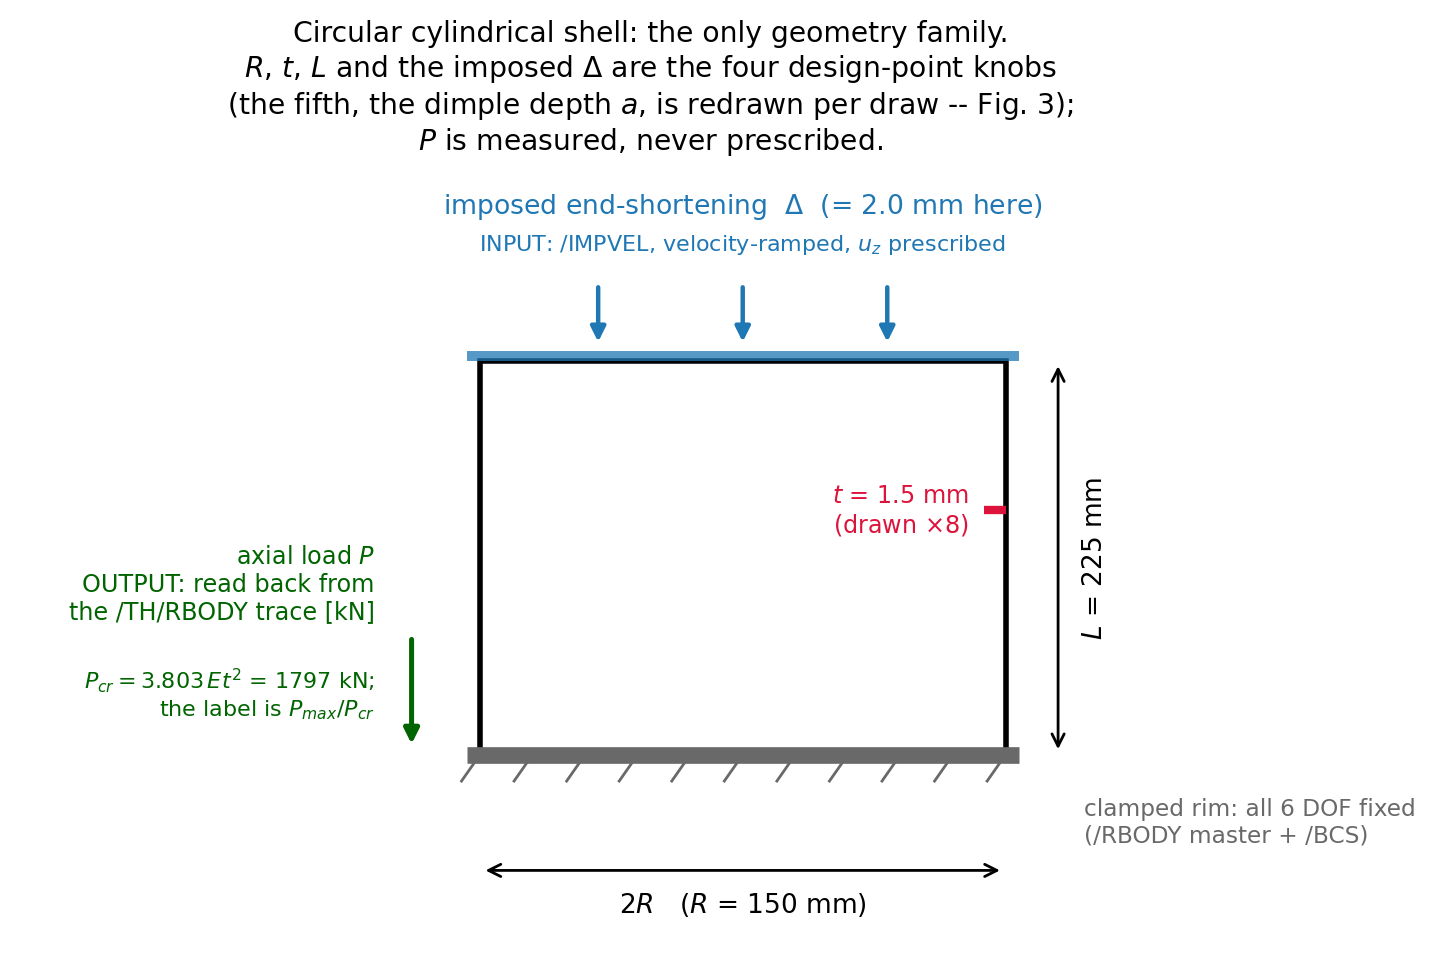
\includegraphics[width=0.9\linewidth]{figures/geometry_schematic.png}
\caption{Boundary conditions, shown at the centre of the design box ($R=150$, $t=1.5$ (drawn
$8\times$ thicker), $L=225$\,mm). The bottom rim is clamped in all six degrees of freedom. The
top rim is driven axially by $\Delta$ at $0.25$\,mm/ms. The reaction force is an output, not an
input. $P_{cr}=3.803\,Et^2$ is 1797\,kN at the centre.}
\label{fig:geom}
\end{figure}

\begin{figure}[!htbp]
\centering
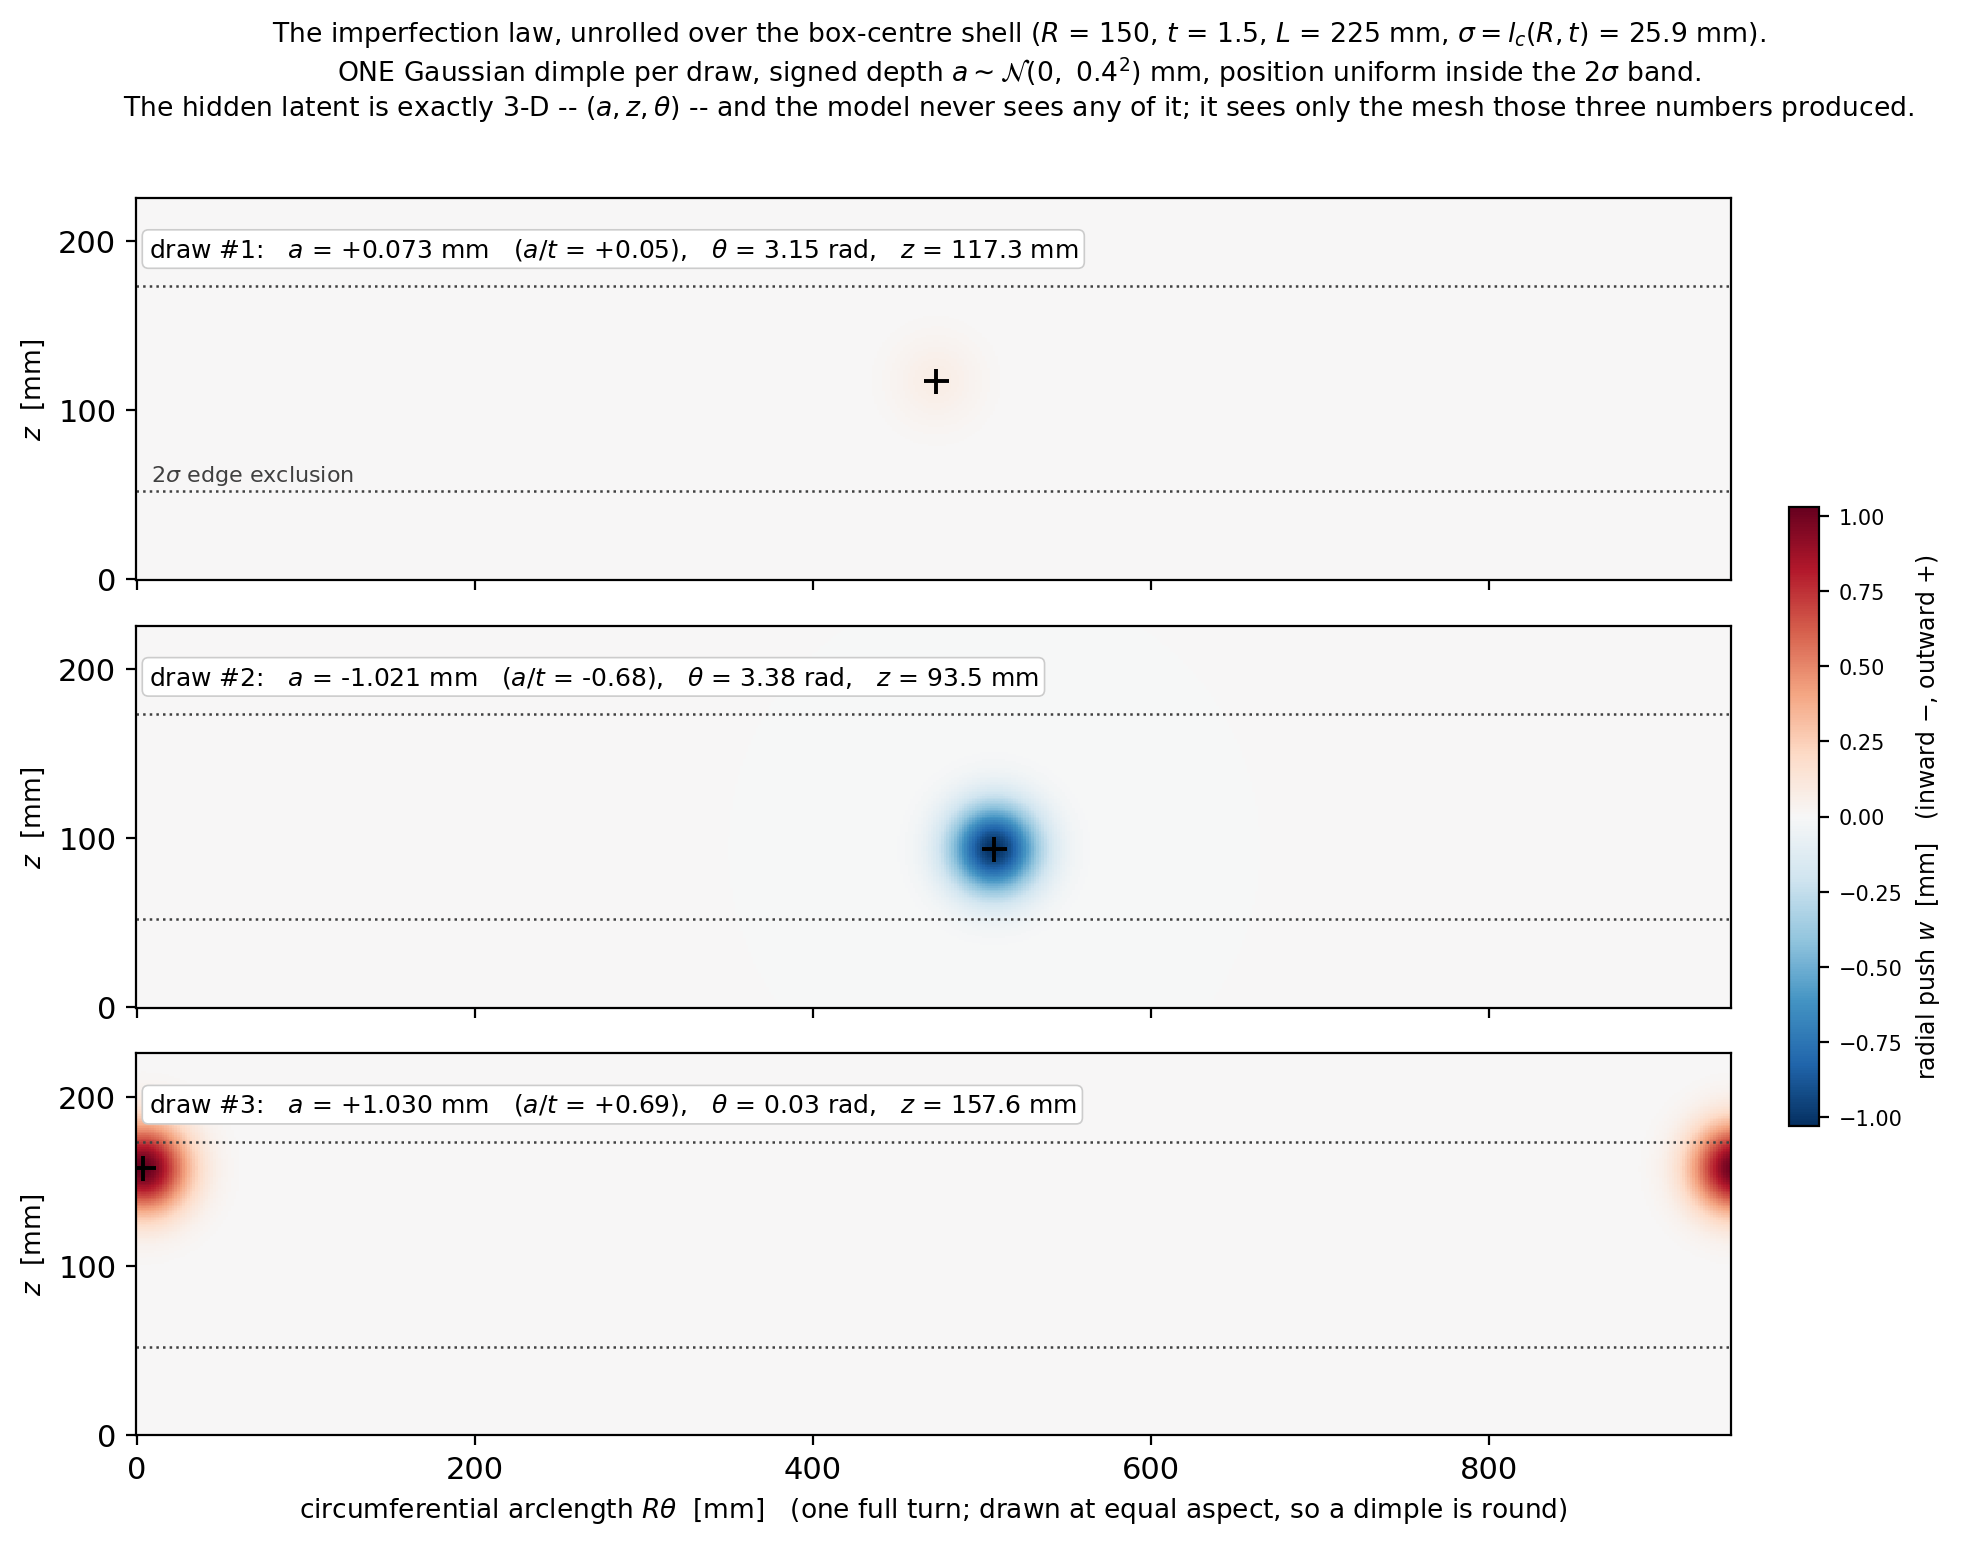
\includegraphics[width=\linewidth]{figures/imperfection_dimples.png}
\caption{The unmeasured input $\xi$. Three samples on the unrolled centre shell ($a=+0.073$, $-1.021$,
$+1.030$\,mm). The dimple width is $\sigma=l_c$ (25.9\,mm at the centre). Its centre is uniform
inside the dashed band, $2\sigma$ away from both rims. The imperfection enters only the
solver's initial geometry; the model input is the nominal cylinder.}
\label{fig:dimples}
\end{figure}

\begin{table}[!htbp]
\centering
\footnotesize
\begin{tabularx}{\textwidth}{@{}l Y@{}}
\toprule
Item & Value \\
\midrule
Design variables & $R\sim U[100,200]$, $t\sim U[1,2]$, $L\sim U[150,300]$, $\Delta\sim U[1,3]$ (mm); 4-D Latin hypercube, 150 geometries \\
Imperfection $\xi$ (not a model input) & 64 samples per geometry; one Gaussian dimple ($K=1$), three random variables: amplitude $a\sim\N(0,0.4^2)$\,mm, uniform angle, axial centre uniform away from a $2\sigma$ band at each rim; width $\sigma=l_c=\pi\sqrt{Rt}/[12(1-\nu^2)]^{1/4}$ \\
Material & linear elastic steel, no yield; $E=210$\,GPa, $\nu=0.3$, $\rho=7.85\times10^{-6}$\,kg/mm$^3$ \\
Elements, mesh & structured quadrilateral shells, 5 through-thickness integration points; $h\le l_c/10$; 27,975--87,398 nodes in training (median 45,409) \\
Solver & OpenRadioss explicit; units kg--mm--ms; terminal kinetic-to-internal energy ratio median 0.034, maximum 0.176 (descriptive, not an acceptance criterion) \\
Boundary conditions & bottom rim clamped (6 DOF); top rim axial velocity $0.25$\,mm/ms to $\Delta$ \\
HDF5 rows & 0:3 coordinates; 3:6 displacement $u$; 6 thickness; 7 $\Delta$; 8 node type \\
Split & by geometry (\code{split_group_attr shape_idx}, seed 42): 120 train / 15 validation / 15 test \\
Common recipes & all 158 geometries (training and out-of-range files) reuse the same 64 imperfection recipes \\
\bottomrule
\end{tabularx}
\caption{Shell-buckling dataset. The imperfection parameters are stored for diagnosis only and
are not model inputs.}
\label{tab:dataset}
\end{table}

\paragraph{Buckling indicator} A draw is counted as buckled when $s=\max_i\|u_i\|$ exceeds
5.17\,mm. The threshold lies between the largest unbuckled and the smallest buckled peak and
agrees with the solver's buckling flag on 97.5\% of the FEA draws.

\paragraph{Where the buckle forms} The dimple seeds the buckle but does not fix where it lies.
In the buckled FE draws of the out-of-range file, the node of largest radial displacement lies
within one dimple width $\sigma$ of the dimple centre, in angle and in axial position, in only
5--27\% of the draws of a geometry, against 1--5\% for a position chosen at random. The radial
lobes above 80\% of the peak cover a median of 6--14 of 18 angular sectors, so a buckle
usually spreads around much of the circumference. In the unbuckled geometry g156 the largest
deviation from the geometry's mean response lies at the dimple in 94\% of the draws. A
buckled field therefore does not reveal its imperfection, and a generated buckled field cannot
be checked by re-running the FE analysis with an imperfection read off the field; criteria
(a) and (b) compare it with independent FE results instead.

\paragraph{Common recipes} The 64 imperfection recipes (amplitude, angle and axial quantile)
are identical across all 158 geometries; the largest difference is $2.6\times10^{-5}$ in the
axial quantile. The test set therefore measures unseen shapes with seen recipes. The
evaluation uses new FE analyses with fresh recipes for every evaluation geometry
(Section~\ref{sec:evalsets}, control A9 in Table~\ref{tab:controls}).

\subsection{Evaluation sets}\label{sec:evalsets}

There are three evaluation sets: 15 unseen test geometries inside the box, 8 near-transition
geometries inside the box ($\lambda\approx0.80$--$0.95$), and 8 geometries that each move one
design variable outside the box. Figure~\ref{fig:eval} shows the test and out-of-range
geometries against the training data, and Table~\ref{tab:ood} lists the out-of-range
geometries. For every evaluation geometry, the reference for (a) and (b) is a new set of 1000 FE analyses
with fresh imperfection recipes, drawn from the same distribution as the training recipes
(control A9); 31 geometries make 31,000 analyses.

\begin{figure}[!htbp]
\centering
\includegraphics[width=\linewidth]{figures/eval_sets.png}
\caption{In-range (training, validation and test) and out-of-range geometries in the four
design variables; the dashed rectangle is the design box. Each out-of-range geometry moves one
variable from the box centre $(150,1.5,225,2.0)$: $R$ 80/240, $t$ 0.8/2.4, $L$ 120/350,
$\Delta$ 0.6/3.6; each panel shows the four that move its variables.}
\label{fig:eval}
\end{figure}

\begin{table}[!htbp]
\centering
\footnotesize
\begin{tabular}{@{}rlrrr@{}}
\toprule
shape & moved variable & $\lambda$ & $P_b$ & nodes \\
\midrule
150 & $R=80$       & 0.783 & 0.41 & 46,224 \\
151 & $R=240$      & 2.350 & 1.00 & 45,982 \\
152 & $t=0.8$      & 2.754 & 1.00 & 85,968 \\
153 & $t=2.4$      & 0.918 & 0.75 & 28,718 \\
154 & $L=120$      & 2.754 & 1.00 & 24,852 \\
155 & $L=350$      & 0.944 & 0.83 & 71,068 \\
156 & $\Delta=0.6$ & 0.441 & 0.00 & 45,780 \\
157 & $\Delta=3.6$ & 2.644 & 1.00 & 45,780 \\
\bottomrule
\end{tabular}
\caption{Out-of-range geometries. $\lambda$: load ratio; $P_b$: FE buckling probability from
the 64 draws of the released file.}
\label{tab:ood}
\end{table}

\paragraph{Provenance of the evaluation draws} The released inference file contains the 8
out-of-range geometries with 64 draws each, generated with the same 64 recipes as the training
set. The analysis of the earlier implementations in Section~\ref{sec:prelim} used an earlier archive with 200
fresh draws per out-of-range and near-transition geometry. That archive, and the
near-transition set as a whole, is not in the released files, so the out-of-range numbers of
Section~\ref{sec:prelim} cannot be reproduced from the released data. The 1000 fresh-recipe
analyses per evaluation geometry replace both, and will be released with the results.

\subsection{Metrics}\label{sec:metrics}

For each geometry, $n_{\text{model}}$ generated fields are compared with the $K$ FE results of
the same geometry. Figure~\ref{fig:diag} shows why the comparison is made geometry by geometry:
within one geometry the peak displacement has two clusters (unbuckled and buckled), and across
geometries the buckling probability goes from 0 to 1 over $\lambda\approx0.6$--$1.05$. The
metrics are grouped by the three criteria of the research gap, after a check that locates
failures and the scalar QoIs that a designer reads.

\begin{figure}[!htbp]
\centering
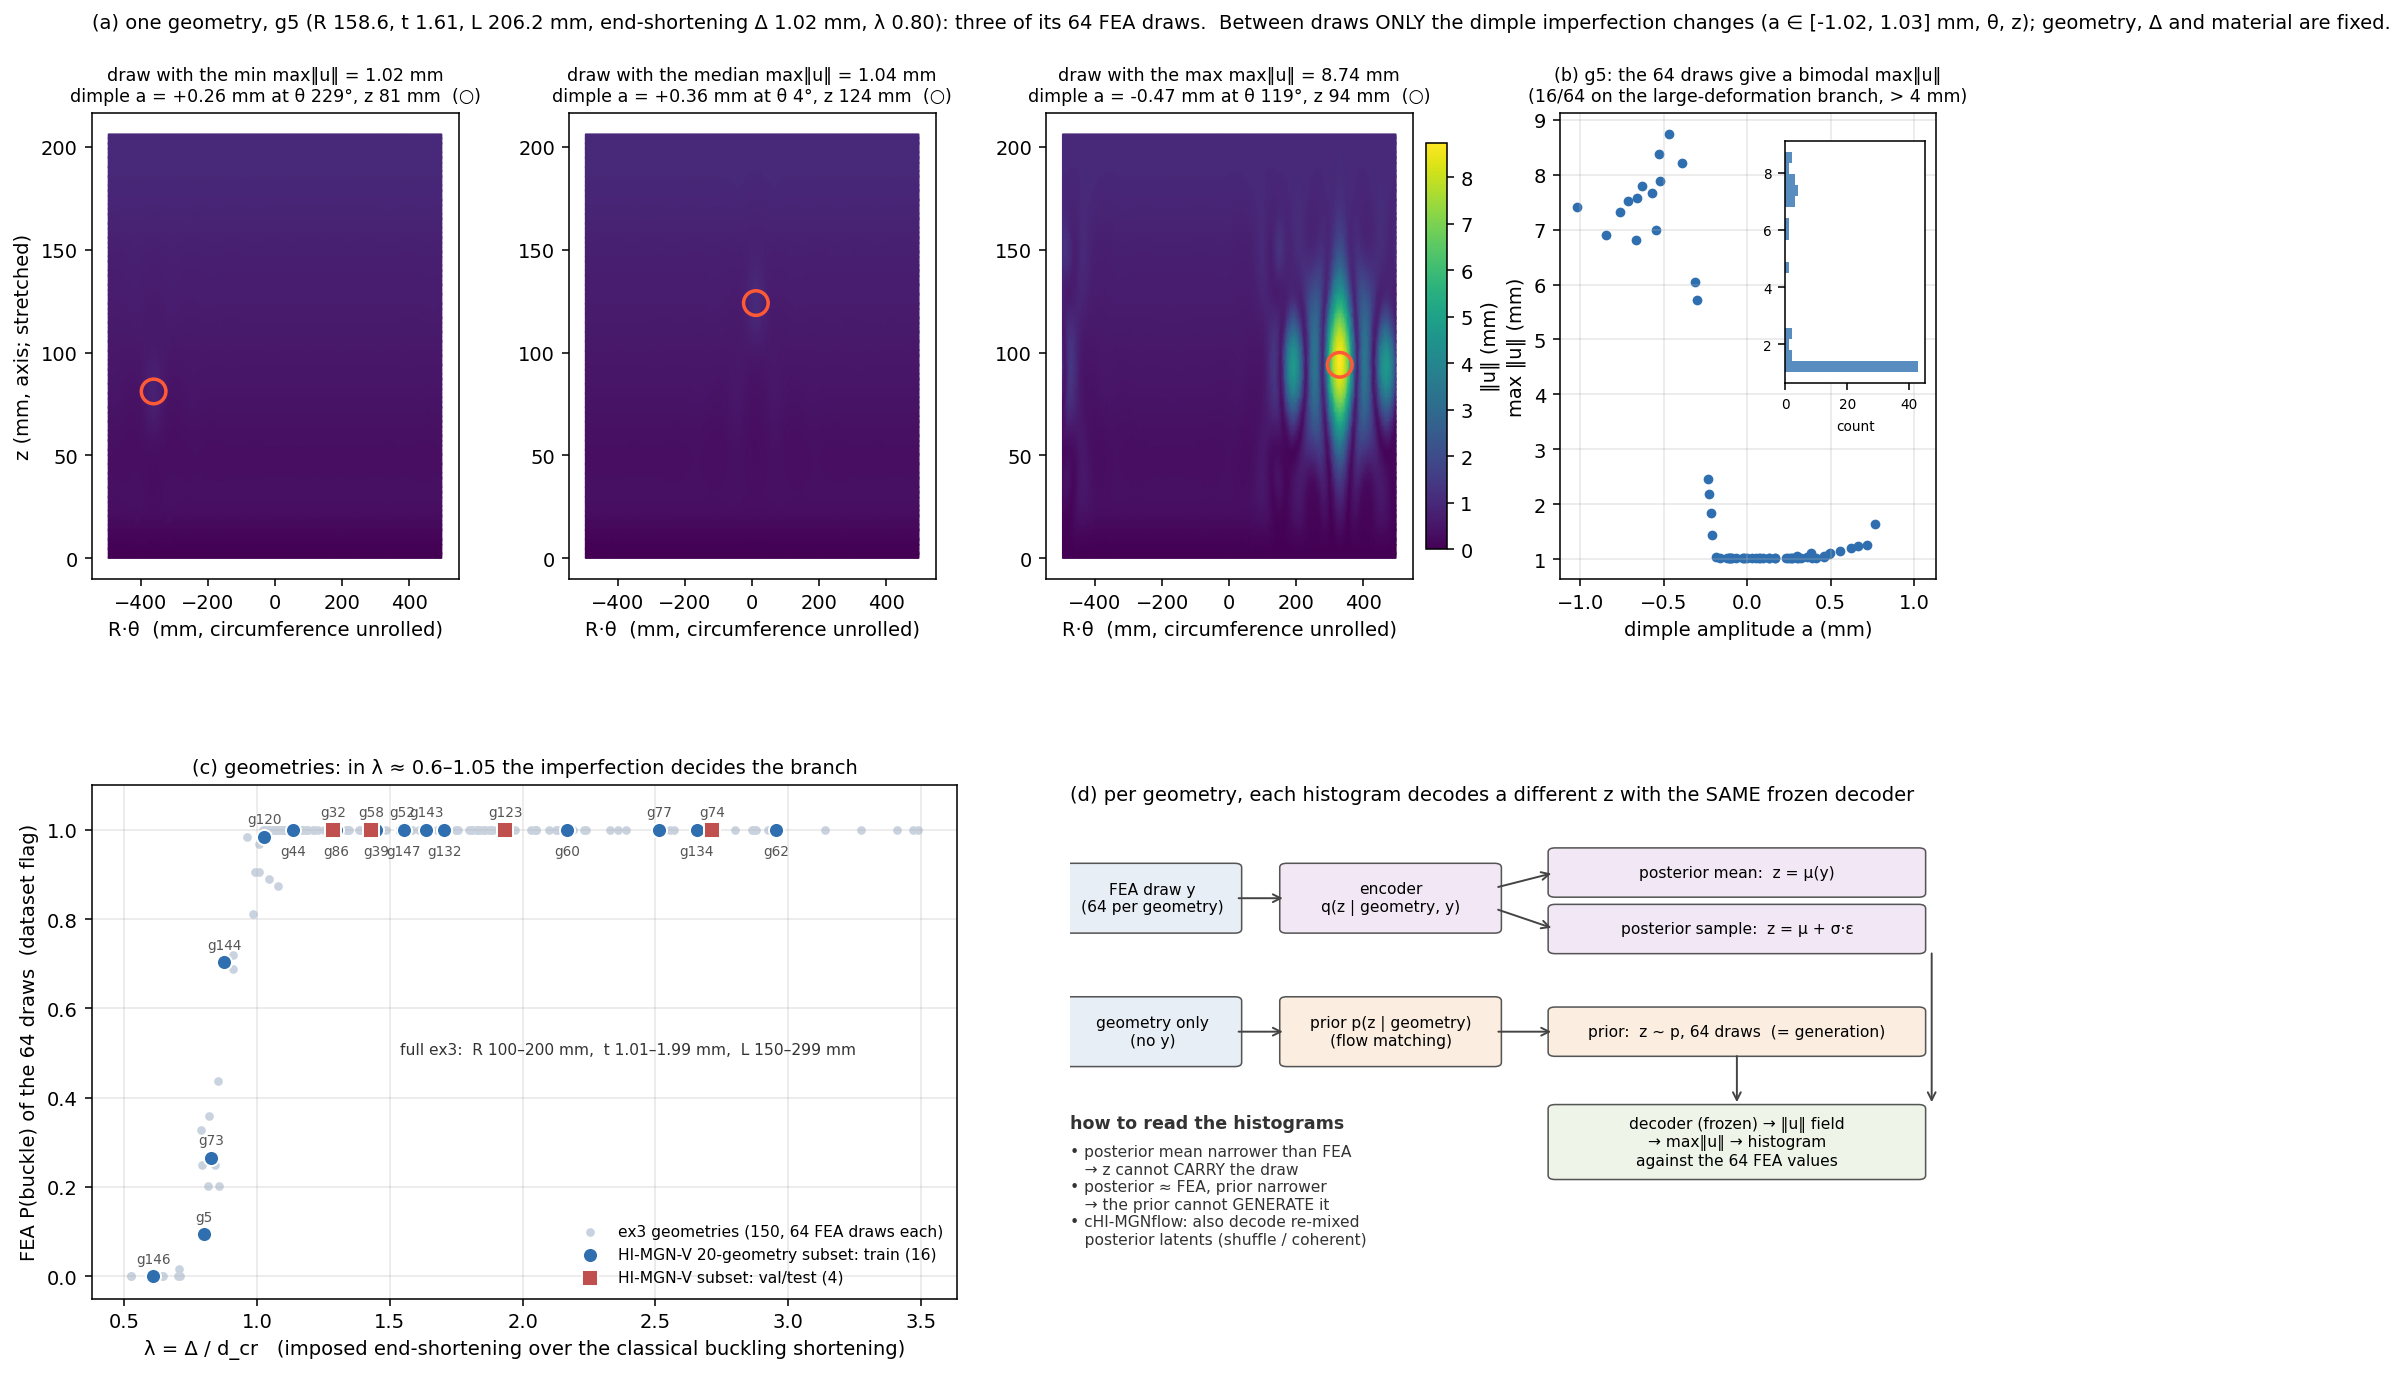
\includegraphics[width=\linewidth]{figures/diag_setup.png}
\caption{Diagnosis setup. (a) Three of the 64 FEA draws of geometry g5 ($\lambda=0.80$); only
the dimple changes between draws. (b) The 64 draws of g5 give a bimodal peak displacement.
(c) FEA buckling probability against $\lambda$ for all 150 geometries; the highlighted points
are a 20-geometry subset used by an earlier run. (d) Posterior-versus-prior check: the same
trained graph network generates fields from latent vectors inferred from the FE results
(posterior mean and posterior draws) and from latent vectors drawn from the learned
distribution (prior), and each set is compared with the FE results.}
\label{fig:diag}
\end{figure}

\paragraph{Posterior versus prior (run first)} The graph network generates two sets of fields
for each geometry: one from latent vectors inferred from the FE results (posterior), one from
latent vectors drawn from the learned distribution (prior). If the first set matches the FE
results and the second does not, the learned distribution is at fault; if both fail, the graph
network or the encoder is. Two further checks mix the regional vectors of different FE results
(shuffled) or keep all of them from one FE result (coherent). This check comes before any
comparison of arms, because it tells which part of the model a difference belongs to.

\paragraph{Scalar QoIs} For the peak displacement $s=\max_i\|u_i\|$: the ratio of the means;
the ratio of the standard deviations $\mathrm{sd}_{\text{model}}/\mathrm{sd}_{\text{FEA}}$
(spread ratio, 1 is correct, below 1 is too little scatter); the Wasserstein distance $W_1$
between the two histograms, which is the average horizontal distance between the two cumulative
distribution curves; the CRPS, which measures the same distance against each FE result in turn;
and the largest vertical gap between the two cumulative curves (Kolmogorov--Smirnov). $W_1$ and
the CRPS are divided by $\mathrm{sd}_{\text{FEA}}$. For the buckling probability: the error
$|P_{\text{model}}-P_{\text{FEA}}|$ and a plot of predicted against FE probability over all
geometries. Results are shown per geometry, as histograms of generated fields beside the FE
results, not only as averaged ratios.

\paragraph{Field distance and rotation} The generated and the FE fields of a geometry live on the
same mesh. For a generated field $\hat\by$ and an FE result $\by$,
\begin{equation}
  R^2(\hat\by\mid\by)=1-\frac{\sum_i\|\hat\by_i-\by_i\|^2}{\sum_i\|\by_i-\bar\by\|^2},\qquad
  d(\hat\by,\by)=\Big(\frac1N\sum_i\|\hat\by_i-\by_i\|^2\Big)^{1/2},
\end{equation}
where $\bar\by$ is the node average of $\by$; the FE result is always the reference. The
cylinder, its boundary conditions and the imperfection distribution are axisymmetric, so an FE
result turned about the axis is an FE result of the same design. The mesh is a structured
lattice with $n_\theta$ nodes per ring, and a turn by a multiple of $2\pi/n_\theta$ is an exact
circular shift of the node indices, with the in-plane displacement components turned with it.
$R^2_{\circlearrowleft}(\hat\by\mid\by)=\max_r R^2(\hat\by\mid Q_r\by)$ takes the best of these turns
$Q_r$.

\paragraph{(a) Sample realism} For each evaluation geometry, $n=1000$ generated fields
$\hat\by_j$ are compared with the $K=1000$ new FE results $\by_k$ in both directions:
\begin{equation}
  A_{\text{real}}=\frac1n\sum_{j}\max_{k}R^2_{\circlearrowleft}(\hat\by_j\mid\by_k),\qquad
  A_{\text{cov}}=\frac1K\sum_{k}\max_{j}R^2_{\circlearrowleft}(\hat\by_j\mid\by_k).
\end{equation}
$A_{\text{real}}$ asks whether every generated field is close to some FE result; it is low for a
model that generates fields between the unbuckled and the buckled state, or buckle lobes no FE
analysis produces. $A_{\text{cov}}$ asks whether every FE result is close to some generated
field; it is low for a model that never generates one kind of FE result, for example the
unbuckled fields of a near-critical design. The first direction is the nearest-state $R^2$ of
LDGN and SAR \cite{lino2025distributions,lino2026sar}; the pair corresponds to precision and
recall \cite{kynkaanniemi2019improved}. The reference value is the leave-one-out score of the FE
results, $A_{\text{FE}}=\frac1K\sum_k\max_{k'\neq k}R^2_{\circlearrowleft}(\by_{k'}\mid\by_k)$,
which a perfect model reaches in both directions with $n=K$. Beside the means, we report the
fraction of generated fields whose nearest-FE $R^2$ is below the 5th percentile of the FE
leave-one-out values (5\% for a perfect model), and the per-geometry histograms of both. The
turn is taken out because (a) asks whether a field is possible, not where around the axis it
lies; the angular distribution is part of (b).

\paragraph{(b) Distribution match} The two sets of fields are compared by the Wasserstein
distance
\begin{equation}
  W_2=\Big(\min_{\pi}\frac1n\sum_{j}d(\hat\by_j,\by_{\pi(j)})^2\Big)^{1/2},
\end{equation}
where $\pi$ runs over the one-to-one assignments of $n$ generated fields to $n$ FE results and
the optimum is found exactly by the Hungarian algorithm on the $n\times n$ distance matrix. In
(a) many generated fields may share one nearest FE result; in $W_2$ each FE result is used
once, so a model that generates one kind of field too often or too rarely leaves fields
matched to distant partners and is penalized, which (a) cannot detect. No turn is taken out: in
the FE results the buckle angle is uniform, and a model that puts every buckle at the same
angle must fail (b). $W_1$ would average the matched distances; $W_2$ is their root mean square,
so a few generated fields far from every FE result weigh more, and it is the distance that LDGN
and SAR report. $W_2$ of finite sets is not zero even for a perfect model, and its bias depends
on $n$. The 1000 FE results of a geometry are therefore split at random into halves A and B of
500: the model score is $W_2$ between 500 generated fields and half A, the reference value
$W_2^{\text{FE}}$ is $W_2$ between half B and half A, and both are averaged over 20 random splits.
We report $W_2$ in mm beside $W_2^{\text{FE}}$ and the ratio $W_2/W_2^{\text{FE}}$, which is 1 for a
model whose fields are distributed as the FE results.

\paragraph{(c) Out-of-range inference} (a), (b) and the scalar QoIs are reported separately on
the test, near-transition and out-of-range sets of Section~\ref{sec:evalsets}.

\paragraph{Buckle position and shape} For buckled fields: the axial and angular position of the
peak, the direction of the peak displacement (inward or outward), the angular extent of the
radial lobes, and the dominant circumferential and axial wavelengths, each compared as a
histogram with the FE results.

\paragraph{Reference values from the FE results alone} With a finite number $K$ of FE results,
even a perfect model does not score zero. Every score is therefore reported beside the value
that FE results alone reach with the same number of samples: the leave-one-out score for (a)
and the split-half score for (b) and for the scalar QoIs
\cite{luthen2023spectral,kansal2023evaluating}. On the existing draws, the split-half mean of
$W_1/\mathrm{sd}$ for $s$ is 0.263, 0.189, 0.151 and 0.144 at $K=16,32,64,100$, and that of
CRPS$/\mathrm{sd}$ about 0.52--0.54. These are comparison points, not lower bounds on what a model
can score.

\paragraph{Statistics} Comparisons are paired on the same geometries, with geometry-level
bootstrap intervals and at least three seeds. A difference between arms is reported as real
only if it exceeds both the seed spread and the bootstrap interval on at least two of the three
sets and does not come with a loss in criterion (a).

\subsection{Baselines, arms and controls}\label{sec:arms}

\paragraph{Baselines} The deterministic HI-MGN gives the mean-response reference. Four
generative baselines produce several fields per geometry: a CVAE on the same V-cycle with a
Gaussian conditional distribution and a KL term \cite{sohn2015cvae}; a generator that adds
random numbers to the deterministic HI-MGN and is trained with the energy score
\cite{shen2025engression,alet2025fgn}; an LDGN-type model that generates a compressed latent
field on the coarse mesh by diffusion \cite{lino2025distributions}; and SAR
\cite{lino2026sar}, run from the authors' released code adapted to the shell data. For SAR,
each geometry is one SAR system and its 64 FE results take the place of the flow states. SAR
receives the same inputs as HI-MGN-V (nominal coordinates, thickness, end shortening and node
type) and generates the final displacement field; the imperfection parameters are not given.
The SAR model, its two training stages (a graph VAE, then scale-by-scale flow matching over the
frozen VAE), its mesh coarsening and its sampler are unchanged, and the hyperparameters are the
authors' wing case. Only the data input, the training loop (plain PyTorch instead of the
authors' training framework, with the same optimizer, learning-rate schedule and stopping
rule), smaller batches with gradient accumulation to the authors' effective batch size, and a
memory-saving but numerically equivalent form of the attention were changed. SAR runs a
network at every mesh level and every integration step, so its cost per generated field is
higher than one pass of HI-MGN-V and is reported. PIFM-GN \cite{song2026pifm} is not included.

\paragraph{Arms} The six HI-MGN-V arms are \{global, local, hybrid\} $\times$ \{MMD, KL\}. They
share every other setting (Appendix~\ref{app:hyper}): training on several GPUs with two
samples per GPU and four accumulation steps in the first phase, learning rate $10^{-4}$, weight
decay $10^{-4}$, 5 warm-up epochs, 120 epochs with the freeze at 80, mixed precision, a running
weight average with factor 0.99, and geometry augmentation. The twelve configuration files (training and inference per arm)
validate under the launcher, and the implementation passes 13 structural tests of shapes,
routing and checkpoint round trips. These tests say nothing about accuracy.

\paragraph{Controls} The arms alone do not separate placement from model size, a random latent
vector from a deterministic global information path, or where the latent vector enters from
where it lives. Table~\ref{tab:controls} lists the
controls.

\begin{table}[!htbp]
\centering
\footnotesize
\begin{tabularx}{\textwidth}{@{}l l Y@{}}
\toprule
ID & Control & What it separates \\
\midrule
A1 & deterministic HI-MGN (MSE) & the value of any random latent vector; the mean-response reference \\
A2 & size-matched arms & placement from parameter count: global vector widened toward $\approx$1024 components, local field narrowed, widths of the learned distributions matched \\
A3 & attribution checks & hold $\zg$ and redraw $\zl$, and the reverse: which part carries which share of the scatter \\
A4 & coarsest level only & the regional vector read at every level versus read once at level 2 \\
A5 & independent distributions & $p(\zg\mid c)\,p(\zl\mid c)$ instead of generating both parts together \\
A6 & known imperfection & the three dimple variables given as inputs and sampled from their known distribution; the unmeasured input revealed \\
A7 & deterministic global vector & a vector of the same width per geometry in the graph network, without randomness: random latent vector versus global information path \\
A8 & $\lambda_{\mathrm{MMD}}=0$ & whether the regularization matters once the distribution is fitted after the freeze \\
A9 & new-imperfection FEA & 1000 new imperfection samples for each of the 31 evaluation geometries: unseen shapes with unseen imperfections, and the reference for (a) and (b) \\
A10 & seeds & at least three training seeds per arm \\
\bottomrule
\end{tabularx}
\caption{Controls. A1, A2, A6, A8 and A10 need only configuration changes or existing tools;
A3--A5 and A7 need new code; A9 needs new FEA.}
\label{tab:controls}
\end{table}

\subsection{Results}\label{sec:prelim}

\paragraph{Results of the unified implementation} No arm of the unified implementation has
been trained at the time of writing. Table~\ref{tab:results} fixes the layout in which the
results will be reported; every entry is pending.

\begin{table}[!htbp]
\centering
\footnotesize
\setlength{\tabcolsep}{2pt}
\begin{tabular}{@{}lcccccccc@{}}
\toprule
& \multicolumn{4}{c}{peak displacement $s$} & \multicolumn{2}{c}{\shortstack{(a) sample\\realism}} & \multicolumn{2}{c}{\shortstack{(b) distrib.\\match}} \\
\cmidrule(lr){2-5}\cmidrule(lr){6-7}\cmidrule(l){8-9}
Model & mean & spread & $W_1/\mathrm{sd}$ & $|\Delta P|$ & $A_{\text{real}}$ & $A_{\text{cov}}$ & $W_2$ & $W_2/W_2^{\text{FE}}$ \\
\midrule
FE vs FE (reference) & 1 & 1 & -- & -- & -- & -- & -- & 1 \\
\midrule
HI-MGN (deterministic) & -- & -- & -- & -- & -- & -- & -- & -- \\
CVAE & -- & -- & -- & -- & -- & -- & -- & -- \\
Energy-score generator & -- & -- & -- & -- & -- & -- & -- & -- \\
LDGN-type & -- & -- & -- & -- & -- & -- & -- & -- \\
SAR (ported) & -- & -- & -- & -- & -- & -- & -- & -- \\
HI-MGN-V global (MMD / KL) & -- & -- & -- & -- & -- & -- & -- & -- \\
HI-MGN-V local (MMD / KL) & -- & -- & -- & -- & -- & -- & -- & -- \\
HI-MGN-V hybrid (MMD / KL) & -- & -- & -- & -- & -- & -- & -- & -- \\
\bottomrule
\end{tabular}
\caption{Layout of the main results, one block per evaluation set (test, near-transition,
out-of-range); the out-of-range block is criterion (c). mean, spread: ratios of
model to FE mean and standard deviation of $s$; $|\Delta P|$: buckling-probability error;
$A_{\text{real}}$, $A_{\text{cov}}$: mean nearest-neighbour $R^2$, generated to FE and FE to
generated; $W_2$ (mm) and its ratio to the FE-alone value. Each block also carries an ``FE vs
FE'' row with the reference values. All entries are pending.}
\label{tab:results}
\end{table}

\paragraph{Earlier implementations} The results below were obtained \emph{before} the
unification, with two separate implementations. ``HI-MGN-V (global)'' is the global placement on
the same graph network. ``HI-MGNflow (regional)'' is a regional model with a different encoder
(it reused the V-cycle features), a KL weight of $10^{-6}$, a first training stage without the
learned distribution, and a separately trained flow-matching distribution on the coarse
clusters. The two differ in more than placement, and the out-of-range and
near-transition sets come from the 200-draw archive described in Section~\ref{sec:evalsets}.
These numbers motivate the method; they are not results of it.

\begin{table}[!htbp]
\centering
\footnotesize
\begin{tabular}{@{}llcccc@{}}
\toprule
Set & Model & mean ratio & spread ratio & $W_1/\mathrm{sd}$ & $|\Delta P|$ \\
\midrule
test (15$\times$64) & HI-MGNflow (regional) & 1.02 & 0.66 & 0.69 & 0.005 \\
 & HI-MGN-V (global) & 0.83 & 1.25 & 1.37 & 0.09 \\
 & \textit{FE vs FE} & & & 0.29 & \\
\midrule
OOD (8$\times$200) & HI-MGNflow (regional) & 1.07 & 0.49 & 0.83 & 0.10 \\
 & HI-MGN-V (global) & 0.80 & 1.06 & 1.63 & 0.16 \\
 & \textit{FE vs FE} & & & 0.14 & \\
\midrule
dense (8$\times$200) & HI-MGNflow (regional) & 1.12 & 0.53 & 0.50 & 0.10 \\
 & HI-MGN-V (global) & 0.63 & 0.66 & 0.56 & 0.28 \\
 & \textit{FE vs FE} & & & 0.11 & \\
\bottomrule
\end{tabular}
\caption{Earlier implementations, peak displacement $s$ per geometry (1000 generated fields
per geometry, averaged over the set). The target for the ratios is 1. $|\Delta P|$ is the
buckling-probability error. ``FE vs FE'' is the reference value from the FE results alone.}
\label{tab:prelim}
\end{table}

\begin{figure}[!htbp]
\centering
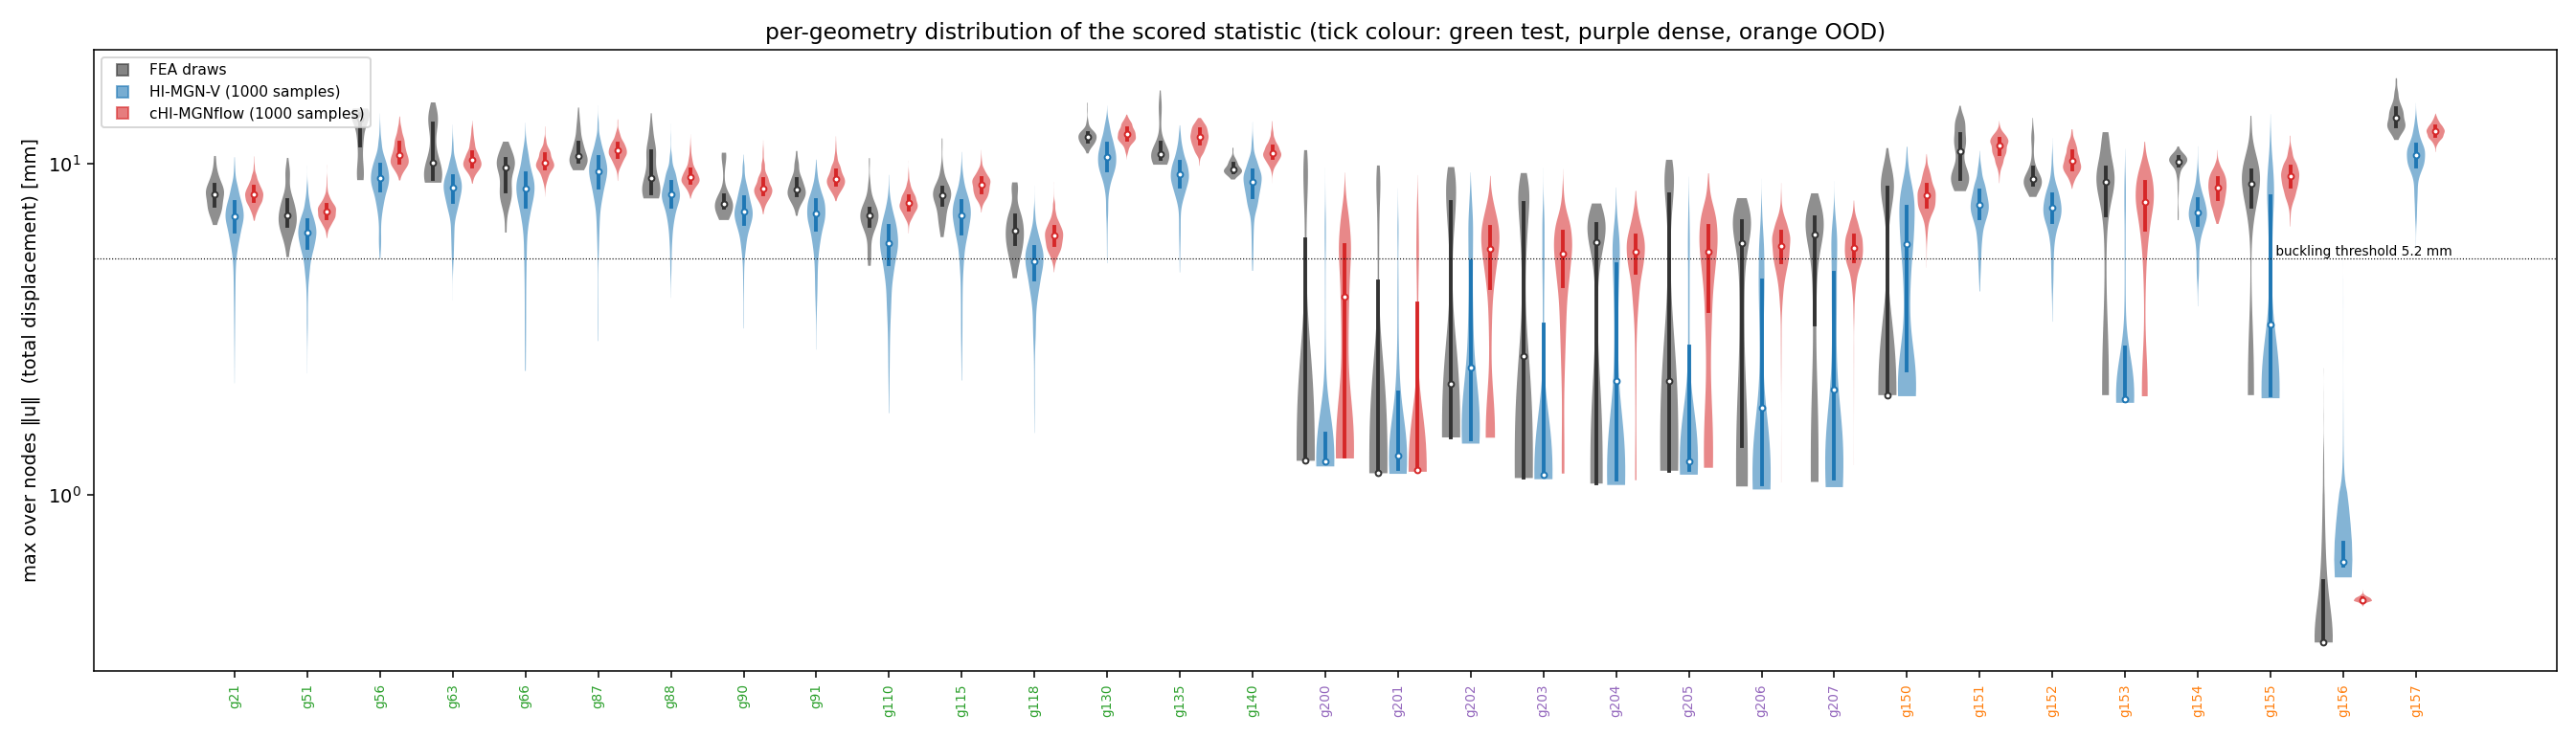
\includegraphics[width=\linewidth]{figures/dense_violins.png}
\caption{Earlier implementations. Per-geometry distributions of the peak displacement (log
axis): FE (grey), the global implementation (blue, labelled HI-MGN-V) and the regional one (red,
labelled with its former name cHI-MGNflow), 1000 samples each. Tick colour: green test, purple
near-transition, orange OOD. The dotted line is the buckling threshold.}
\label{fig:violins}
\end{figure}

\begin{figure}[!htbp]
\centering
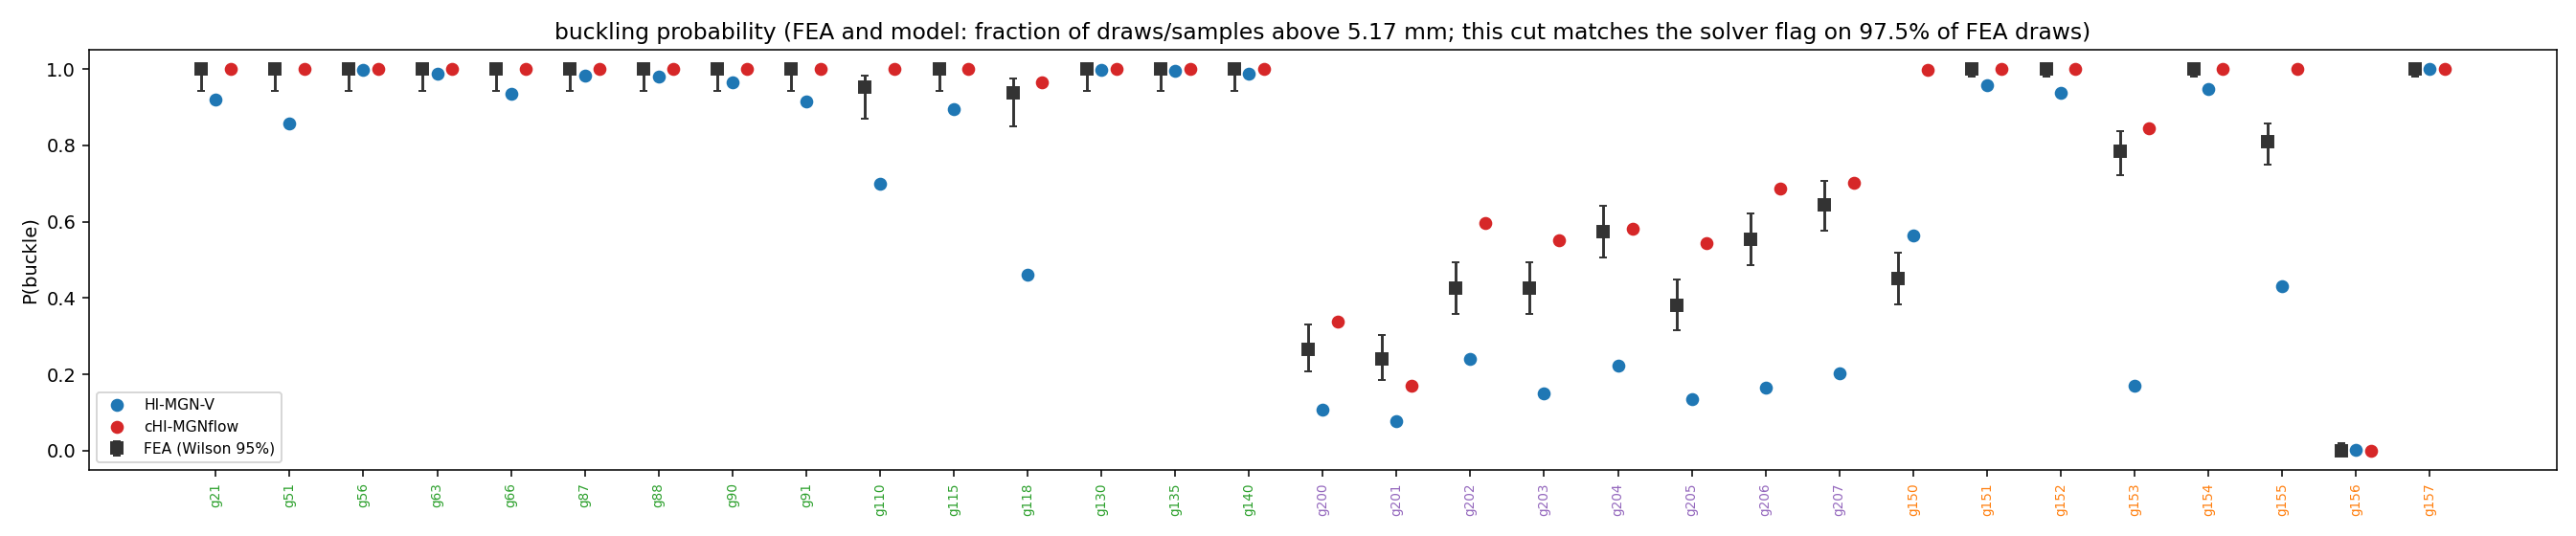
\includegraphics[width=\linewidth]{figures/dense_pbuckle.png}
\caption{Earlier implementations. Buckling probability per geometry: FE with Wilson 95\%
intervals; models as the fraction of generated fields above 5.17\,mm.}
\label{fig:pbuckle}
\end{figure}

\paragraph{Observations}
\begin{enumerate}
\item \emph{The two placements fail in opposite directions.} The regional model has the right
  mean (mean ratio 1.02--1.12) but too little scatter (spread ratio 0.49--0.66), and it predicts
  buckling where FE gives a mix (g150: 1.00 against 0.45). The global model underestimates the
  displacement (0.63--0.83). Its spread ratio above one on the test set comes from a long tail of
  unbuckled fields where FE buckles, not from a correct scatter (Figure~\ref{fig:violins}), and
  it predicts too few buckled shells near the transition (0.08--0.24 against FE 0.24--0.65 on
  the near-transition set).
\item \emph{Where the error sits.} In the regional model, fields generated from latent vectors
  inferred from the FE results (posterior) reach a spread ratio of 0.97, fields from the learned
  distribution (prior) 0.57, shuffled regional vectors 0.48 and coherent ones 0.97: the learned
  distribution, not the graph network, loses the scatter. Making it four times deeper (4 to 16
  blocks) moved the spread ratio only from 0.59 to 0.62, and the first three principal
  components of its fields carry 0.42--0.51 of the FE variance. In the global model, the
  amplitude of the fields generated from the posterior mean is 0.56--0.81 of the FE value and the
  latent vector explains about 47\% of the scatter, so the global vector does not carry enough
  information to tell the 64 FE results of a geometry apart.
\item \emph{The ranking is not the same on every geometry.} On geometry g150 the global model
  is far closer ($W_1/\mathrm{sd}$ 0.34 against 0.93). Later parameter studies moved both: a
  wider regional distribution network (width 128) removed the regional bias, and for the global
  model only a ten-fold MMD weight helped.
\end{enumerate}

The pattern is the starting hypothesis for the placement statement of
Section~\ref{sec:placement}. A regional latent field reproduces where the response localizes
but not how often the shell buckles; a global latent vector carries a shared variable but not
enough spatial detail. Whether a hybrid, with both parts generated together, does better than
either at the same model size is what the unified study tests.

%======================================================================
\section{Discussion and limitations}\label{sec:discussion}

\paragraph{What each outcome would mean} If the hybrid beats both single placements at the
same model size (A2) and loses that gain when its two parts are generated independently (A5),
the gain comes from generating them together. If the deterministic global vector (A7) closes
the gap to the hybrid, the global part helps by passing information across the structure, not
by its randomness. If reading the regional vector at the coarsest level only (A4) works as well
as reading it at every level, the every-level reading of Table~\ref{tab:placement} is
unnecessary; if it fails, it is needed. If the model that is given the imperfection (A6) is far
ahead of every arm, the difficulty is inferring the effect of $\xi$ from the field, not the
graph network. If no HI-MGN-V arm beats the energy-score generator, the latent vector and its
learned distribution are not needed for this problem.

\paragraph{Why the distribution is fitted after a freeze} The regional implementation showed
that a distribution trained together with the encoder chases a moving target and ends with too
little scatter. Fitting it to the latent vectors of the frozen encoder, after scaling, removes
the moving target. LSGM reports the opposite trade-off for images \cite{vahdat2021lsgm}. The
first phase still trains the distribution, so it starts the second phase from a good state,
but its gradient does not change the encoder.

\paragraph{What the regularization can and cannot do} MMD makes the set of all inferred
latent vectors look like a standard normal distribution, per level vector or per channel. It
does not limit how much each vector says about its FE result, which suits a graph network that
should use the latent vector. KL limits this for every sample and can make a weak latent vector
carry no information \cite{higgins2017beta}. In both cases the dependence on the nominal input
is carried by the distribution fitted after the freeze. The six arms measure which
regularization leaves latent vectors that this distribution can fit.

\paragraph{Limitations}
\begin{itemize}
\item No result of the unified implementation is reported. Section~\ref{sec:prelim} uses
  earlier implementations that differ in more than placement.
\item One dataset, with one dimple per analysis. Several interacting imperfections, material
  scatter or load scatter may favour another placement.
\item All geometries, including the released out-of-range file, reuse the same 64 imperfection
  recipes, so the test measures unseen shapes with seen imperfections. The 200-sample archive
  behind the earlier out-of-range and near-transition numbers is not in the released files. The
  1000 fresh-recipe analyses per evaluation geometry that the protocol needs (31,000 in all,
  about three times the training campaign) have not been run.
\item A buckled field does not reveal its imperfection (Section~\ref{sec:dataset}), so a
  generated field is scored against independent FE results, not against a re-analysis of
  its own imperfection.
\item The clusters are random. Regional latent vectors do not correspond to physical regions,
  and a model may depend on the node numbering through the first seed node.
\item The default arms are not capacity-matched (Table~\ref{tab:params}).
\item The global MMD is estimated on a batch of two samples per GPU, and the local MMD ignores
  the correlation between clusters (Section~\ref{sec:reg}).
\item The peak-to-valley term acts on the axial displacement, not on the scored QoI
  (Section~\ref{sec:training}).
\item The objective is not a likelihood bound, so no likelihood comparison is possible.
\end{itemize}

\paragraph{Claims this paper does not make} Table~\ref{tab:noclaims} lists phrasings we avoid
and why.

\begin{table}[!htbp]
\centering
\footnotesize
\begin{tabularx}{\textwidth}{@{}Y Y@{}}
\toprule
Not claimed & Reason / correct statement \\
\midrule
``first to address one-to-many responses in mechanics'' & stochastic emulators, CVAEs, Gen-Fab, GUST, Han \& Bahmani, equivariant flow matching and Bi-FORK address parts of it (Table~\ref{tab:ox}) \\
``first generative surrogate on meshes'' & LDGN, SAR, PIFM-GN and Graph-EFM exist \\
``first hybrid latent'' & LION, DualDiff, HPU-Net and others combine global and local latent variables \\
``first to evaluate sample realism, distribution match and out-of-range inference'' & only after (a)--(c) are computed, and limited to structural fields with scatter from an unmeasured input \\
``the diffusion-transformer conditioning (AdaLN-Zero)'' & there is no normalization and the gate starts at one: a gated FiLM \\
``ELBO'' or ``likelihood'' & the loss is a weighted sum; MMD acts on the set of latent vectors, not on each one \\
``regional latent vectors are physical regions'' & the clusters are random \\
``a global random vector helps'' & a hypothesis, pending the deterministic-global control (A7) \\
``the method works outside the training range'' & out-of-range geometries are \emph{evaluated}; too little scatter and a biased mean were observed in the earlier implementations \\
\bottomrule
\end{tabularx}
\caption{Wording constraints applied throughout.}
\label{tab:noclaims}
\end{table}

%======================================================================
\section{Conclusion}\label{sec:conclusion}

When an input of the manufactured part is not measured, a structural surrogate has to
generate the scatter of response fields, not one field. Existing field surrogates in mechanics
are deterministic, generative surrogates on meshes reproduce the time variation of turbulent
flows, and surrogates of input scatter return scalar or low-dimensional outputs. HI-MGN-V
generates complete response fields on unstructured FE meshes from the nominal design: a
multilevel graph network whose blocks are adjusted by a latent vector drawn from a learned
distribution conditioned on the design. Whether the latent vector acts globally, regionally or
both is a stated assumption about how the unmeasured input acts, and it is one setting of one
implementation. The evaluation compares generated fields with many FE analyses of the same
design on three criteria: (a) sample realism, every generated field is close to some FE
result and every FE result to some generated field; (b) distribution match, the generated fields
are distributed as the FE results, by a Wasserstein distance read against the value that FE
results alone reach; and (c) out-of-range inference, both hold outside the training range. The test problem is a shell-buckling dataset in which the unmeasured imperfection
decides whether the shell buckles. Earlier implementations of the global and local options fail
in opposite ways on this dataset, which motivates the hybrid and the controlled study that will
test it.

\appendix
\section{Hyperparameters}\label{app:hyper}

\begin{table}[!htbp]
\centering
\footnotesize
\begin{tabularx}{\textwidth}{@{}l Y@{}}
\toprule
Group & Setting \\
\midrule
Data & \code{input_var 3}, \code{output_var 3}, \code{cond_var 2}, \code{use_node_types}, \code{positional_features 4}, \code{edge_var 8}, \code{augment_geometry}, \code{split_group_attr shape_idx}, \code{split_seed 42} \\
Training & DDP; batch 2, \code{grad_accum_steps 4} (joint phase); lr $10^{-4}$; weight decay $10^{-4}$; warm-up 5; 120 epochs; AMP; checkpointing; EMA 0.99; \code{training_seed 42}; \code{best_by crps} with \code{vae_valid_prior_samples} 8 (default) \\
Graph network & \code{latent_dim 128}; \code{message_passing_num 15}; \code{use_multiscale}; \code{coarsening_type voronoi_seedmean}; \code{multiscale_levels 2}; \code{voronoi_clusters 4096, 256}; \code{mp_per_level 2,3,5,3,2}; \code{hierarchy_variants 2}; \code{hierarchy_seed 42} \\
Latent & \code{latent_type global|local|hybrid}; \code{vae_latent_dim 32} (3 levels); \code{latent_ch 4}; \code{vae_mp_layers 3}; \code{vae_local_mp_layers 2}; \code{vae_graph_aware}; \code{posterior_min_std 0.05}; \code{z_conditioning adaln} \\
Loss & \code{alpha_recon 1000} (MSE); \code{latent_reg mmd} ($\lambda=1$) or \code{kl} (\code{kl_weight 1e-3}); \code{beta_aux 10} (peak-to-valley, axial channel); \code{prior_nll_weight 1}; \code{prior_grad_to_encoder 0} \\
Learned distribution & \code{use_conditional_prior}; \code{prior_type gnn_e2e}; \code{prior_family fm}; \code{prior_mp_layers 3}; \code{prior_hidden_dim 128}; coarse prior 4 blocks; \code{prior_fm_steps 30}; \code{prior_fm_solver heun}; \code{prior_freeze_epoch 80} \\
Inference & 64 samples per geometry in the configuration files, 1000 for the evaluation protocol; spread statistic \code{mag_max} on channels 0--2 \\
\bottomrule
\end{tabularx}
\caption{Settings shared by the six arms (\nolinkurl{configs/MeshGraphNets_Variational/probabilistic/ex3/latent_type/}). Only \code{latent_type} and \code{latent_reg} (with its weight) differ.}
\label{tab:hyper}
\end{table}

\bibliographystyle{elsarticle-num}
\bibliography{references}

\end{document}
